% Options for packages loaded elsewhere
% Options for packages loaded elsewhere
\PassOptionsToPackage{unicode}{hyperref}
\PassOptionsToPackage{hyphens}{url}
\PassOptionsToPackage{dvipsnames,svgnames,x11names}{xcolor}
%
\documentclass[
  letterpaper,
  DIV=11,
  numbers=noendperiod]{scrartcl}
\usepackage{xcolor}
\usepackage{amsmath,amssymb}
\setcounter{secnumdepth}{5}
\usepackage{iftex}
\ifPDFTeX
  \usepackage[T1]{fontenc}
  \usepackage[utf8]{inputenc}
  \usepackage{textcomp} % provide euro and other symbols
\else % if luatex or xetex
  \usepackage{unicode-math} % this also loads fontspec
  \defaultfontfeatures{Scale=MatchLowercase}
  \defaultfontfeatures[\rmfamily]{Ligatures=TeX,Scale=1}
\fi
\usepackage{lmodern}
\ifPDFTeX\else
  % xetex/luatex font selection
\fi
% Use upquote if available, for straight quotes in verbatim environments
\IfFileExists{upquote.sty}{\usepackage{upquote}}{}
\IfFileExists{microtype.sty}{% use microtype if available
  \usepackage[]{microtype}
  \UseMicrotypeSet[protrusion]{basicmath} % disable protrusion for tt fonts
}{}
\makeatletter
\@ifundefined{KOMAClassName}{% if non-KOMA class
  \IfFileExists{parskip.sty}{%
    \usepackage{parskip}
  }{% else
    \setlength{\parindent}{0pt}
    \setlength{\parskip}{6pt plus 2pt minus 1pt}}
}{% if KOMA class
  \KOMAoptions{parskip=half}}
\makeatother
% Make \paragraph and \subparagraph free-standing
\makeatletter
\ifx\paragraph\undefined\else
  \let\oldparagraph\paragraph
  \renewcommand{\paragraph}{
    \@ifstar
      \xxxParagraphStar
      \xxxParagraphNoStar
  }
  \newcommand{\xxxParagraphStar}[1]{\oldparagraph*{#1}\mbox{}}
  \newcommand{\xxxParagraphNoStar}[1]{\oldparagraph{#1}\mbox{}}
\fi
\ifx\subparagraph\undefined\else
  \let\oldsubparagraph\subparagraph
  \renewcommand{\subparagraph}{
    \@ifstar
      \xxxSubParagraphStar
      \xxxSubParagraphNoStar
  }
  \newcommand{\xxxSubParagraphStar}[1]{\oldsubparagraph*{#1}\mbox{}}
  \newcommand{\xxxSubParagraphNoStar}[1]{\oldsubparagraph{#1}\mbox{}}
\fi
\makeatother

\usepackage{color}
\usepackage{fancyvrb}
\newcommand{\VerbBar}{|}
\newcommand{\VERB}{\Verb[commandchars=\\\{\}]}
\DefineVerbatimEnvironment{Highlighting}{Verbatim}{commandchars=\\\{\}}
% Add ',fontsize=\small' for more characters per line
\usepackage{framed}
\definecolor{shadecolor}{RGB}{241,243,245}
\newenvironment{Shaded}{\begin{snugshade}}{\end{snugshade}}
\newcommand{\AlertTok}[1]{\textcolor[rgb]{0.68,0.00,0.00}{#1}}
\newcommand{\AnnotationTok}[1]{\textcolor[rgb]{0.37,0.37,0.37}{#1}}
\newcommand{\AttributeTok}[1]{\textcolor[rgb]{0.40,0.45,0.13}{#1}}
\newcommand{\BaseNTok}[1]{\textcolor[rgb]{0.68,0.00,0.00}{#1}}
\newcommand{\BuiltInTok}[1]{\textcolor[rgb]{0.00,0.23,0.31}{#1}}
\newcommand{\CharTok}[1]{\textcolor[rgb]{0.13,0.47,0.30}{#1}}
\newcommand{\CommentTok}[1]{\textcolor[rgb]{0.37,0.37,0.37}{#1}}
\newcommand{\CommentVarTok}[1]{\textcolor[rgb]{0.37,0.37,0.37}{\textit{#1}}}
\newcommand{\ConstantTok}[1]{\textcolor[rgb]{0.56,0.35,0.01}{#1}}
\newcommand{\ControlFlowTok}[1]{\textcolor[rgb]{0.00,0.23,0.31}{\textbf{#1}}}
\newcommand{\DataTypeTok}[1]{\textcolor[rgb]{0.68,0.00,0.00}{#1}}
\newcommand{\DecValTok}[1]{\textcolor[rgb]{0.68,0.00,0.00}{#1}}
\newcommand{\DocumentationTok}[1]{\textcolor[rgb]{0.37,0.37,0.37}{\textit{#1}}}
\newcommand{\ErrorTok}[1]{\textcolor[rgb]{0.68,0.00,0.00}{#1}}
\newcommand{\ExtensionTok}[1]{\textcolor[rgb]{0.00,0.23,0.31}{#1}}
\newcommand{\FloatTok}[1]{\textcolor[rgb]{0.68,0.00,0.00}{#1}}
\newcommand{\FunctionTok}[1]{\textcolor[rgb]{0.28,0.35,0.67}{#1}}
\newcommand{\ImportTok}[1]{\textcolor[rgb]{0.00,0.46,0.62}{#1}}
\newcommand{\InformationTok}[1]{\textcolor[rgb]{0.37,0.37,0.37}{#1}}
\newcommand{\KeywordTok}[1]{\textcolor[rgb]{0.00,0.23,0.31}{\textbf{#1}}}
\newcommand{\NormalTok}[1]{\textcolor[rgb]{0.00,0.23,0.31}{#1}}
\newcommand{\OperatorTok}[1]{\textcolor[rgb]{0.37,0.37,0.37}{#1}}
\newcommand{\OtherTok}[1]{\textcolor[rgb]{0.00,0.23,0.31}{#1}}
\newcommand{\PreprocessorTok}[1]{\textcolor[rgb]{0.68,0.00,0.00}{#1}}
\newcommand{\RegionMarkerTok}[1]{\textcolor[rgb]{0.00,0.23,0.31}{#1}}
\newcommand{\SpecialCharTok}[1]{\textcolor[rgb]{0.37,0.37,0.37}{#1}}
\newcommand{\SpecialStringTok}[1]{\textcolor[rgb]{0.13,0.47,0.30}{#1}}
\newcommand{\StringTok}[1]{\textcolor[rgb]{0.13,0.47,0.30}{#1}}
\newcommand{\VariableTok}[1]{\textcolor[rgb]{0.07,0.07,0.07}{#1}}
\newcommand{\VerbatimStringTok}[1]{\textcolor[rgb]{0.13,0.47,0.30}{#1}}
\newcommand{\WarningTok}[1]{\textcolor[rgb]{0.37,0.37,0.37}{\textit{#1}}}

\usepackage{longtable,booktabs,array}
\usepackage{calc} % for calculating minipage widths
% Correct order of tables after \paragraph or \subparagraph
\usepackage{etoolbox}
\makeatletter
\patchcmd\longtable{\par}{\if@noskipsec\mbox{}\fi\par}{}{}
\makeatother
% Allow footnotes in longtable head/foot
\IfFileExists{footnotehyper.sty}{\usepackage{footnotehyper}}{\usepackage{footnote}}
\makesavenoteenv{longtable}
\usepackage{graphicx}
\makeatletter
\newsavebox\pandoc@box
\newcommand*\pandocbounded[1]{% scales image to fit in text height/width
  \sbox\pandoc@box{#1}%
  \Gscale@div\@tempa{\textheight}{\dimexpr\ht\pandoc@box+\dp\pandoc@box\relax}%
  \Gscale@div\@tempb{\linewidth}{\wd\pandoc@box}%
  \ifdim\@tempb\p@<\@tempa\p@\let\@tempa\@tempb\fi% select the smaller of both
  \ifdim\@tempa\p@<\p@\scalebox{\@tempa}{\usebox\pandoc@box}%
  \else\usebox{\pandoc@box}%
  \fi%
}
% Set default figure placement to htbp
\def\fps@figure{htbp}
\makeatother





\setlength{\emergencystretch}{3em} % prevent overfull lines

\providecommand{\tightlist}{%
  \setlength{\itemsep}{0pt}\setlength{\parskip}{0pt}}



 


\KOMAoption{captions}{tableheading}
\makeatletter
\@ifpackageloaded{tcolorbox}{}{\usepackage[skins,breakable]{tcolorbox}}
\@ifpackageloaded{fontawesome5}{}{\usepackage{fontawesome5}}
\definecolor{quarto-callout-color}{HTML}{909090}
\definecolor{quarto-callout-note-color}{HTML}{0758E5}
\definecolor{quarto-callout-important-color}{HTML}{CC1914}
\definecolor{quarto-callout-warning-color}{HTML}{EB9113}
\definecolor{quarto-callout-tip-color}{HTML}{00A047}
\definecolor{quarto-callout-caution-color}{HTML}{FC5300}
\definecolor{quarto-callout-color-frame}{HTML}{acacac}
\definecolor{quarto-callout-note-color-frame}{HTML}{4582ec}
\definecolor{quarto-callout-important-color-frame}{HTML}{d9534f}
\definecolor{quarto-callout-warning-color-frame}{HTML}{f0ad4e}
\definecolor{quarto-callout-tip-color-frame}{HTML}{02b875}
\definecolor{quarto-callout-caution-color-frame}{HTML}{fd7e14}
\makeatother
\makeatletter
\@ifpackageloaded{caption}{}{\usepackage{caption}}
\AtBeginDocument{%
\ifdefined\contentsname
  \renewcommand*\contentsname{Table of contents}
\else
  \newcommand\contentsname{Table of contents}
\fi
\ifdefined\listfigurename
  \renewcommand*\listfigurename{List of Figures}
\else
  \newcommand\listfigurename{List of Figures}
\fi
\ifdefined\listtablename
  \renewcommand*\listtablename{List of Tables}
\else
  \newcommand\listtablename{List of Tables}
\fi
\ifdefined\figurename
  \renewcommand*\figurename{Figure}
\else
  \newcommand\figurename{Figure}
\fi
\ifdefined\tablename
  \renewcommand*\tablename{Table}
\else
  \newcommand\tablename{Table}
\fi
}
\@ifpackageloaded{float}{}{\usepackage{float}}
\floatstyle{ruled}
\@ifundefined{c@chapter}{\newfloat{codelisting}{h}{lop}}{\newfloat{codelisting}{h}{lop}[chapter]}
\floatname{codelisting}{Listing}
\newcommand*\listoflistings{\listof{codelisting}{List of Listings}}
\makeatother
\makeatletter
\makeatother
\makeatletter
\@ifpackageloaded{caption}{}{\usepackage{caption}}
\@ifpackageloaded{subcaption}{}{\usepackage{subcaption}}
\makeatother
\usepackage{bookmark}
\IfFileExists{xurl.sty}{\usepackage{xurl}}{} % add URL line breaks if available
\urlstyle{same}
\hypersetup{
  pdftitle={Hypothesis Testing},
  colorlinks=true,
  linkcolor={blue},
  filecolor={Maroon},
  citecolor={Blue},
  urlcolor={Blue},
  pdfcreator={LaTeX via pandoc}}


\title{Hypothesis Testing}
\usepackage{etoolbox}
\makeatletter
\providecommand{\subtitle}[1]{% add subtitle to \maketitle
  \apptocmd{\@title}{\par {\large #1 \par}}{}{}
}
\makeatother
\subtitle{Lecture 7}
\author{}
\date{}
\begin{document}
\maketitle


\section{Outline}\label{outline}

\begin{itemize}
\tightlist
\item
  What is Hypothesis Testing?
\item
  Elements of a Statistical Test
\item
  What are p-values?
\item
  Tests of Means
\item
  Tests of Proportions
\end{itemize}

\section{Hypothesis Testing}\label{hypothesis-testing}

\subsection{What is Hypothesis
Testing?}\label{what-is-hypothesis-testing}

Recall that confidence intervals are used to provide interval estimates
for the population parameter. Often, we want to ask if the parameters
behave a specific way.

\begin{tcolorbox}[enhanced jigsaw, bottomtitle=1mm, colback=white, opacityback=0, leftrule=.75mm, opacitybacktitle=0.6, coltitle=black, left=2mm, colframe=quarto-callout-important-color-frame, toptitle=1mm, colbacktitle=quarto-callout-important-color!10!white, titlerule=0mm, title=\textcolor{quarto-callout-important-color}{\faExclamation}\hspace{0.5em}{Important}, arc=.35mm, rightrule=.15mm, breakable, bottomrule=.15mm, toprule=.15mm]

Examples of research questions we might ask are:

\begin{itemize}
\tightlist
\item
  Is the mean lifetime of a person using a newly developed drug the same
  as the lifetime with a standard drug?
\item
  Is the mortality rate equal to 1\%?
\end{itemize}

\end{tcolorbox}

\subsection{Hypothesis Testing
Example}\label{hypothesis-testing-example}

Consider the mean lifetime example. Suppose you perform the study and
you find that the average lifetime for the newly developed drug is 35
years, while those with the standard drug had an average lifetime of 34
years.

\begin{tcolorbox}[enhanced jigsaw, bottomtitle=1mm, colback=white, opacityback=0, leftrule=.75mm, opacitybacktitle=0.6, coltitle=black, left=2mm, colframe=quarto-callout-note-color-frame, toptitle=1mm, colbacktitle=quarto-callout-note-color!10!white, titlerule=0mm, title=\textcolor{quarto-callout-note-color}{\faInfo}\hspace{0.5em}{Note}, arc=.35mm, rightrule=.15mm, breakable, bottomrule=.15mm, toprule=.15mm]

Could this difference of 1 year easily have occurred by chance even if
the drugs work the same?

\end{tcolorbox}

\begin{tcolorbox}[enhanced jigsaw, bottomtitle=1mm, colback=white, opacityback=0, leftrule=.75mm, opacitybacktitle=0.6, coltitle=black, left=2mm, colframe=quarto-callout-important-color-frame, toptitle=1mm, colbacktitle=quarto-callout-important-color!10!white, titlerule=0mm, title=\textcolor{quarto-callout-important-color}{\faExclamation}\hspace{0.5em}{Important}, arc=.35mm, rightrule=.15mm, breakable, bottomrule=.15mm, toprule=.15mm]

We need to determine the probability of observing at least a 1-year
difference in average lifetimes between the two groups under the
assumption that the population means are equal.

\begin{itemize}
\tightlist
\item
  If this probability is high, then it's not unlikely to observe a
  1-year difference or more due to randomness.
\item
  If this probability is low, then it's unlikely to observe a 1-year
  difference or more due to randomness. There is evidence that Drug A
  works better than Drug B.
\end{itemize}

\end{tcolorbox}

\section{Elements of a Statistical Hypothesis
Test}\label{elements-of-a-statistical-hypothesis-test}

\subsection{Statistical Hypothesis}\label{statistical-hypothesis}

In general, a statistical hypothesis is a statement about one or more
parameters.

\begin{tcolorbox}[enhanced jigsaw, bottomtitle=1mm, colback=white, opacityback=0, leftrule=.75mm, opacitybacktitle=0.6, coltitle=black, left=2mm, colframe=quarto-callout-warning-color-frame, toptitle=1mm, colbacktitle=quarto-callout-warning-color!10!white, titlerule=0mm, title=\textcolor{quarto-callout-warning-color}{\faExclamationTriangle}\hspace{0.5em}{Warning}, arc=.35mm, rightrule=.15mm, breakable, bottomrule=.15mm, toprule=.15mm]

The statistical hypothesis is aligned with the \emph{research
hypothesis}, but not exactly the same. The research hypothesis addresses
the problem stated for the study, but it does not need to provide a
statemment about the parameters.

\end{tcolorbox}

\subsection{Types of Statistical
Hypotheses}\label{types-of-statistical-hypotheses}

There are two types of statistical hypotheses: the null and alternative
hypotheses.

\begin{tcolorbox}[enhanced jigsaw, bottomtitle=1mm, colback=white, opacityback=0, leftrule=.75mm, opacitybacktitle=0.6, coltitle=black, left=2mm, colframe=quarto-callout-note-color-frame, toptitle=1mm, colbacktitle=quarto-callout-note-color!10!white, titlerule=0mm, title=\textcolor{quarto-callout-note-color}{\faInfo}\hspace{0.5em}{Null Hypothesis}, arc=.35mm, rightrule=.15mm, breakable, bottomrule=.15mm, toprule=.15mm]

The null hypothesis, \(H_0\), is usually a specific statement about the
parameters and is the statement against which we seek evidence.

\end{tcolorbox}

\begin{tcolorbox}[enhanced jigsaw, bottomtitle=1mm, colback=white, opacityback=0, leftrule=.75mm, opacitybacktitle=0.6, coltitle=black, left=2mm, colframe=quarto-callout-note-color-frame, toptitle=1mm, colbacktitle=quarto-callout-note-color!10!white, titlerule=0mm, title=\textcolor{quarto-callout-note-color}{\faInfo}\hspace{0.5em}{Alternative Hypothesis}, arc=.35mm, rightrule=.15mm, breakable, bottomrule=.15mm, toprule=.15mm]

The alternative hypothesis, \(H_a\), is the statement that we conclude
if we decide against the null hypothesis.

\end{tcolorbox}

\subsection{Null Hypotheses}\label{null-hypotheses}

The null hypothesis is often a statement about the parameters that
amount to nothing or random chance.

\begin{tcolorbox}[enhanced jigsaw, bottomtitle=1mm, colback=white, opacityback=0, leftrule=.75mm, opacitybacktitle=0.6, coltitle=black, left=2mm, colframe=quarto-callout-note-color-frame, toptitle=1mm, colbacktitle=quarto-callout-note-color!10!white, titlerule=0mm, title=\textcolor{quarto-callout-note-color}{\faInfo}\hspace{0.5em}{Note}, arc=.35mm, rightrule=.15mm, breakable, bottomrule=.15mm, toprule=.15mm]

The null hypothesis could be that two treatments may yield the same
mean, mortality rate remains the same, a coin is fair, or two random
variables are not associated with each other.

\end{tcolorbox}

\begin{tcolorbox}[enhanced jigsaw, bottomtitle=1mm, colback=white, opacityback=0, leftrule=.75mm, opacitybacktitle=0.6, coltitle=black, left=2mm, colframe=quarto-callout-important-color-frame, toptitle=1mm, colbacktitle=quarto-callout-important-color!10!white, titlerule=0mm, title=\textcolor{quarto-callout-important-color}{\faExclamation}\hspace{0.5em}{Important}, arc=.35mm, rightrule=.15mm, breakable, bottomrule=.15mm, toprule=.15mm]

Consider the mean lifetime example. The null hypothesis corresponds to
the scenario that both treatment and standard groups yield the same
average lifetimes. The parameter of interest is then the difference in
population average lifetime between the two groups. Explicitly,

\(H_0\): The average lifetime of the treatment group is equal to the
average lifetime of the standard group.

\[
H_0: \mu_{trt} - \mu_{standard} = 0
\]

\end{tcolorbox}

\subsection{Alternative Hypothesis}\label{alternative-hypothesis}

The alternative hypothesis \(H_a\) is the statement that we conclude if
we decide against the null hypothesis. Often, the null and alternative
hypothesis should cover the entire parameter space.

\subsubsection{Warning}

\begin{tcolorbox}[enhanced jigsaw, bottomtitle=1mm, colback=white, opacityback=0, leftrule=.75mm, opacitybacktitle=0.6, coltitle=black, left=2mm, colframe=quarto-callout-warning-color-frame, toptitle=1mm, colbacktitle=quarto-callout-warning-color!10!white, titlerule=0mm, title=\textcolor{quarto-callout-warning-color}{\faExclamationTriangle}\hspace{0.5em}{Warning}, arc=.35mm, rightrule=.15mm, breakable, bottomrule=.15mm, toprule=.15mm]

However, there are times when the two hypotheses only cover a part of
the parameter space depending on what convention is used for the null
hypothesis.

\end{tcolorbox}

\subsubsection{Example}

Consider the mean lifetime example. If we were looking for evidence that
the treatment performs better than the standard drug in increasing
lifetimes, then that would be our alternative hypothesis. Explicitly,

\(H_a:\) The population average lifetime of the treatment group is
higher than the average lifetime of the treatment group.

\[
H_a: \mu_{trt} -\mu_{standard} >0
\]

\subsubsection{Notes}

The hypotheses can be expressed by the following statements:

\[
H_0: \mu_{trt} - \mu_{standard} = 0
\]

\[
H_a: \mu_{trt} -\mu_{standard} >0
\]

These values do \textbf{NOT} span the entire parameter space
\((-\infty,\infty)\). Rather it only considers one side. Hence, \(H_a\)
is considered as a one-sided hypothesis.

\begin{tcolorbox}[enhanced jigsaw, bottomtitle=1mm, colback=white, opacityback=0, leftrule=.75mm, opacitybacktitle=0.6, coltitle=black, left=2mm, colframe=quarto-callout-tip-color-frame, toptitle=1mm, colbacktitle=quarto-callout-tip-color!10!white, titlerule=0mm, title=\textcolor{quarto-callout-tip-color}{\faLightbulb}\hspace{0.5em}{Tip}, arc=.35mm, rightrule=.15mm, breakable, bottomrule=.15mm, toprule=.15mm]

There are references who would express the null hypothesis as
\(\mu_{trt}-\mu_{standard} \leq 0\). The case
\(\mu_{trt}-\mu_{standard} < 0\) means the treatment works worse than
the placebo, implying the drug is not effective.

\textbf{In this course}, we will be as specific as possible when
choosing \(H_0\) by \textbf{only retaining the equality in the null
hypothesis}.

\end{tcolorbox}

\subsection{Example}\label{example-1}

Suppose we want to see whether there was evidence that the germination
rate of seeds planted in a new soil mix formulation was higher than
70\%.

\subsubsection{Question}

What are the null and alternative hypotheses for this study?

\subsubsection{Answer}

\(H_0:\) The long-run germination rate of seeds planted in the new soil
mix is equal to 70\%

\[
H_0: \pi_{germination} = 0.70
\]

\(H_a:\) The long-run germination rate of seeds planted in the new soil
mix is higher than 70\%

\[
H_a: \pi_{germination} > 0.70
\]

\subsection{Example}\label{example-2}

Suppose we want to disprove the claim that the average single-serving
sugar content of a brand of dark chocolate is 3 grams.

\subsubsection{Question}

What are the null and alternative hypotheses for this study?

\subsubsection{Answer}

\(H_0:\) The population average single-serving sugar content of a brand
of dark chocolate is equal to 3 grams. OR The long-run average
single-serving sugar content of a brand of dark chocolate is equal to 3
grams.

\[
H_0: \mu = 3
\]

\(H_a:\) The population average single-serving sugar content of a brand
of dark chocolate is \emph{NOT} equal to 3 grams. OR The long-run
average single-serving sugar content of a brand of dark chocolate is
\emph{NOT} equal to 3 grams.

\[
H_a: \mu \neq 3
\]

\subsection{Exercise}\label{exercise}

Consider the following studies:

\begin{enumerate}
\def\labelenumi{\arabic{enumi}.}
\item
  Researchers were interested in determining whether the daily average
  amount of dog food in their local animal shelter was lower than 500
  grams.
\item
  Suppose a design company created two designs (A and B) for the website
  of a new community clinic. The clinic administrators wanted to test
  whether there was a difference in proportion of site visitors who
  preferred each design.
\end{enumerate}

\subsubsection{Questions}

What are the parameters of interest? What are the null and alternative
hypotheses for these studies?

\subsubsection{Answer 1}

Parameter of interest: Long-run daily average amount of dog food
\(H_0:\) The long-run daily average amount of dog food is equal to 500
grams. \(H_a:\) The long-run daily average amount of dog food is less
than 500 grams.

\[
H_0: \mu = 500; H_a: \mu < 500
\]

\subsubsection{Answer 2}

\(H_0:\) There is no difference in proportion of site visitors who
preferred Designs A and B. \(H_a:\) There is a difference in proportion
of site visitors who preferred Designs A and B.

\[
H_0: \pi_A - \pi_B = 0; H_a: \pi_A-\pi_B \neq 0
\]

\subsection{Hypothesis Testing:
Decisions}\label{hypothesis-testing-decisions}

The main idea behind hypothesis testing is to \textbf{assume the null
hypothesis is true until we get evidence that it is false.}

\begin{tcolorbox}[enhanced jigsaw, bottomtitle=1mm, colback=white, opacityback=0, leftrule=.75mm, opacitybacktitle=0.6, coltitle=black, left=2mm, colframe=quarto-callout-note-color-frame, toptitle=1mm, colbacktitle=quarto-callout-note-color!10!white, titlerule=0mm, title=\textcolor{quarto-callout-note-color}{\faInfo}\hspace{0.5em}{Note}, arc=.35mm, rightrule=.15mm, breakable, bottomrule=.15mm, toprule=.15mm]

How do we get evidence that \(H_0\) is false? If the probability of
obtaining the measured statistic (or more extreme values) assuming the
null hypothesis is low, then this is evidence \textbf{against} the null
hypothesis.

How low should this probability be?

\end{tcolorbox}

\begin{tcolorbox}[enhanced jigsaw, bottomtitle=1mm, colback=white, opacityback=0, leftrule=.75mm, opacitybacktitle=0.6, coltitle=black, left=2mm, colframe=quarto-callout-important-color-frame, toptitle=1mm, colbacktitle=quarto-callout-important-color!10!white, titlerule=0mm, title=\textcolor{quarto-callout-important-color}{\faExclamation}\hspace{0.5em}{Important}, arc=.35mm, rightrule=.15mm, breakable, bottomrule=.15mm, toprule=.15mm]

Once we've established this threshold, we need to make a
\emph{decision}.

\begin{itemize}
\tightlist
\item
  Reject \(H_0\)
\item
  Do Not Reject \(H_0\) (Note: Failing to Reject \(H_0\) is not the same
  as accepting \(H_0\)).
\end{itemize}

\end{tcolorbox}

\subsection{Error Types and Significance
Level}\label{error-types-and-significance-level}

\subsubsection{Errors}

There is no error when the null hypothesis is rejected when it is false
and when the null hypothesis is not rejected when it is true. However,
the following cases are errors:

\begin{tcolorbox}[enhanced jigsaw, bottomtitle=1mm, colback=white, opacityback=0, leftrule=.75mm, opacitybacktitle=0.6, coltitle=black, left=2mm, colframe=quarto-callout-note-color-frame, toptitle=1mm, colbacktitle=quarto-callout-note-color!10!white, titlerule=0mm, title=\textcolor{quarto-callout-note-color}{\faInfo}\hspace{0.5em}{Type I error}, arc=.35mm, rightrule=.15mm, breakable, bottomrule=.15mm, toprule=.15mm]

A Type I error occurs when the null hypothesis is rejected when it is
true.

\end{tcolorbox}

\begin{tcolorbox}[enhanced jigsaw, bottomtitle=1mm, colback=white, opacityback=0, leftrule=.75mm, opacitybacktitle=0.6, coltitle=black, left=2mm, colframe=quarto-callout-note-color-frame, toptitle=1mm, colbacktitle=quarto-callout-note-color!10!white, titlerule=0mm, title=\textcolor{quarto-callout-note-color}{\faInfo}\hspace{0.5em}{Type II error}, arc=.35mm, rightrule=.15mm, breakable, bottomrule=.15mm, toprule=.15mm]

A Type II error occurs when the null hypothesis is not rejected when it
is false.

\end{tcolorbox}

\subsubsection{Error Tables}

\pandocbounded{\includegraphics[keepaspectratio]{lecture7_files/mediabag/Type-I-and-type-II-E.jpg}}

\subsubsection{Significance Level}

Type I errors cannot be avoided due to the randomness of the process.
The standard approach in hypothesis testing is to determine the cutoff
point for our decision so that the probability of making a Type I error
is some small predetermined number. This number is referred to as the
\textbf{significance level}, \(\alpha\). Formally,

\[
\alpha = P(Reject~H_0|True~H_0) = P(Type~I~Error)
\]

The most common value used for the significance level is
\(\alpha = 0.05\).

\subsection{Hypothesis Testing:
Terminology}\label{hypothesis-testing-terminology}

\begin{tcolorbox}[enhanced jigsaw, bottomtitle=1mm, colback=white, opacityback=0, leftrule=.75mm, opacitybacktitle=0.6, coltitle=black, left=2mm, colframe=quarto-callout-note-color-frame, toptitle=1mm, colbacktitle=quarto-callout-note-color!10!white, titlerule=0mm, title=\textcolor{quarto-callout-note-color}{\faInfo}\hspace{0.5em}{Test Statistic}, arc=.35mm, rightrule=.15mm, breakable, bottomrule=.15mm, toprule=.15mm]

The \emph{test statistic} is some function of the data that is used to
make the decision about whether to reject \(H_0\) or fail to reject
\(H_0\).

\end{tcolorbox}

\begin{tcolorbox}[enhanced jigsaw, bottomtitle=1mm, colback=white, opacityback=0, leftrule=.75mm, opacitybacktitle=0.6, coltitle=black, left=2mm, colframe=quarto-callout-note-color-frame, toptitle=1mm, colbacktitle=quarto-callout-note-color!10!white, titlerule=0mm, title=\textcolor{quarto-callout-note-color}{\faInfo}\hspace{0.5em}{Rejection Region}, arc=.35mm, rightrule=.15mm, breakable, bottomrule=.15mm, toprule=.15mm]

The \emph{rejection region}, also called the \emph{critical region}, is
the set of values of the test statistic that lead us to reject \(H_0\).

\end{tcolorbox}

\subsection{Example: Basic Hypothesis
Testing}\label{example-basic-hypothesis-testing}

Suppose that a hospital emergency department sees patients with
influenza-like illness (ILI) at an average rate of six per day, except
when there is a flu outbreak, in which case the rate is higher. Each
day, the hospital records the number of ILI cases and tests whether
there is evidence of an outbreak.

\subsubsection{Questions}

\begin{itemize}
\tightlist
\item
  What should the null and alternative hypotheses be for testing whether
  there is evidence of an outbreak?
\item
  What is the rejection region corresponding to a significance level
  \(\alpha=0.05\).
\item
  Do we have evidence of an outbreak when we receive a count of 12 cases
  for a single day?
\end{itemize}

\subsubsection{Answers}

Since we're dealing with counts, we will use the Poisson distribution to
describe the distribution of the number of cases. The hypothesis should
be related to the rate parameter \(\lambda\).

\[
H_0: \lambda=6; H_a: \lambda > 6
\] where \(\lambda\) is the average daily count of ILI cases. To find
the rejection region, we need to find the critical value \(x_c\) such
that \(P(X \geq x_c) <= 0.05\) (choose the value with the highest
probability to fit this criteria).

\begin{Shaded}
\begin{Highlighting}[]
\FunctionTok{library}\NormalTok{(tidyverse)}
\end{Highlighting}
\end{Shaded}

\begin{verbatim}
-- Attaching core tidyverse packages ------------------------ tidyverse 2.0.0 --
v dplyr     1.1.4     v readr     2.1.5
v forcats   1.0.0     v stringr   1.5.1
v ggplot2   3.5.2     v tibble    3.3.0
v lubridate 1.9.4     v tidyr     1.3.1
v purrr     1.1.0     
-- Conflicts ------------------------------------------ tidyverse_conflicts() --
x dplyr::filter() masks stats::filter()
x dplyr::lag()    masks stats::lag()
i Use the conflicted package (<http://conflicted.r-lib.org/>) to force all conflicts to become errors
\end{verbatim}

\begin{Shaded}
\begin{Highlighting}[]
\NormalTok{df }\OtherTok{\textless{}{-}} \FunctionTok{data.frame}\NormalTok{(}\AttributeTok{xc=}\DecValTok{6}\SpecialCharTok{:}\DecValTok{15}\NormalTok{)}
\NormalTok{df2 }\OtherTok{\textless{}{-}} \FunctionTok{mutate}\NormalTok{(df, }\AttributeTok{probs =} \DecValTok{1}\SpecialCharTok{{-}}\FunctionTok{ppois}\NormalTok{(xc,}\AttributeTok{lambda=}\DecValTok{6}\NormalTok{))}
\NormalTok{df2}
\end{Highlighting}
\end{Shaded}

\begin{verbatim}
   xc        probs
1   6 0.3936972176
2   7 0.2560202395
3   8 0.1527625060
4   9 0.0839240170
5  10 0.0426209236
6  11 0.0200919635
7  12 0.0088274835
8  13 0.0036284927
9  14 0.0014003538
10 15 0.0005090983
\end{verbatim}

The data frame shows that when \(x_c=10\), \(P(X \geq 10) = 0.0426\),
which is lower than 0.05. This means the rejection/critical region is
\(X\geq 10\). If we get at least 10 cases, we have evidence of an
outbreak. If we get less than 10 cases, we have no evidence of an
outbreak.

\subsection{Power}\label{power}

Power is the probability of rejecting the null hypothesis when the null
hypothesis is false.

\begin{tcolorbox}[enhanced jigsaw, bottomtitle=1mm, colback=white, opacityback=0, leftrule=.75mm, opacitybacktitle=0.6, coltitle=black, left=2mm, colframe=quarto-callout-important-color-frame, toptitle=1mm, colbacktitle=quarto-callout-important-color!10!white, titlerule=0mm, title=\textcolor{quarto-callout-important-color}{\faExclamation}\hspace{0.5em}{Important}, arc=.35mm, rightrule=.15mm, breakable, bottomrule=.15mm, toprule=.15mm]

The concept of power is closely related to sample size selection. In
hypothesis testing, the sample size is determined so that the power at a
fixed value of the alternative hypothesis is equal to a predetermined
value or based on a set effect size.

\end{tcolorbox}

\subsection{p-values}\label{p-values}

\begin{tcolorbox}[enhanced jigsaw, bottomtitle=1mm, colback=white, opacityback=0, leftrule=.75mm, opacitybacktitle=0.6, coltitle=black, left=2mm, colframe=quarto-callout-important-color-frame, toptitle=1mm, colbacktitle=quarto-callout-important-color!10!white, titlerule=0mm, title=\textcolor{quarto-callout-important-color}{\faExclamation}\hspace{0.5em}{Important}, arc=.35mm, rightrule=.15mm, breakable, bottomrule=.15mm, toprule=.15mm]

The p-value is the probability of getting a test statistic as extreme or
more extreme than what was actually observed given that \(H_0\) is true.
``More extreme'' refers to getting a test statistic further away from
the cutoff point that determines the rejection region.

The smaller p-value, the stronger the evidence against the null
hypothesis \(H_0\).

\end{tcolorbox}

\begin{tcolorbox}[enhanced jigsaw, bottomtitle=1mm, colback=white, opacityback=0, leftrule=.75mm, opacitybacktitle=0.6, coltitle=black, left=2mm, colframe=quarto-callout-important-color-frame, toptitle=1mm, colbacktitle=quarto-callout-important-color!10!white, titlerule=0mm, title=\textcolor{quarto-callout-important-color}{\faExclamation}\hspace{0.5em}{Important}, arc=.35mm, rightrule=.15mm, breakable, bottomrule=.15mm, toprule=.15mm]

p-values are also often used for hypothesis testing to decide whether to
reject \(H_0\) or not. A common rule is to \textbf{reject the null
hypothesis when the p-value is less than the significance level}
\(\alpha\), and fail to reject otherwise.

An alternative definition of the p-value is that the p-value is the
smallest value of \(\alpha\) that leads to the rejection of the null
hypothesis.

\end{tcolorbox}

\subsection{Example: p-values}\label{example-p-values}

Suppose that a hospital emergency department sees patients with
influenza-like illness (ILI) at an average rate of six per day, except
when there is a flu outbreak, in which case the rate is higher. Each
day, the hospital records the number of ILI cases and tests whether
there is evidence of an outbreak.

\subsubsection{Questions}

Recall that the hypotheses are given by

\[
H_0: \lambda = 6; H_a: \lambda > 6
\]

Calculate the p-value if the daily number of ILI cases was 12.

\subsubsection{Answer}

Assuming the null hypothesis is true, we assume \(\lambda =6\). We need
to calculate the probability of getting a count as extreme or more
extreme than 6, i.e.~further away from 6. Therefore, we need to
calculate the \(P(X \geq 12)\) using a Poisson distribution with
\(\lambda=6\).

\begin{Shaded}
\begin{Highlighting}[]
\NormalTok{prob }\OtherTok{\textless{}{-}} \DecValTok{1}\SpecialCharTok{{-}}\FunctionTok{ppois}\NormalTok{(}\DecValTok{11}\NormalTok{,}\AttributeTok{lambda=}\DecValTok{6}\NormalTok{)}
\NormalTok{prob}
\end{Highlighting}
\end{Shaded}

\begin{verbatim}
[1] 0.02009196
\end{verbatim}

The resulting p-value is p=0.020092.

After seeing this result, you must believe one of two things.

\begin{itemize}
\tightlist
\item
  \(H_0\) is true and you observed an event with probability 0.0201
\item
  \(H_0\) is false.
\end{itemize}

\subsection{Hypothesis Testing:
Approach}\label{hypothesis-testing-approach}

The approach for hypothesis testing can be described as follows:

\begin{itemize}
\tightlist
\item
  Determine the parameter of interest
\item
  Determine the appropriate null and alternative hypotheses
\item
  Choose a value for the significance level.
\item
  Determine the rejection region.
\item
  Compute the test statistic
\item
  If the test statistic is in the rejection region, then reject the null
  hypothesis; otherwise, fail to reject the null hypothesis.
\end{itemize}

\section{Tests Involving Means}\label{tests-involving-means}

\subsection{Hypothesis Test: Single Mean, Known
Variance}\label{hypothesis-test-single-mean-known-variance}

Suppose now that we observe a sample from a Gaussian distribution with
known variance \(\sigma^2\). If we are interested in testing the null
hypothesis \(H_0: \mu=\mu_0\), the alternative hypothesis can be one of
the following:

\begin{itemize}
\tightlist
\item
  One-sided hypotheses: \(H_a: \mu < \mu_0\) or \(H_a: \mu > \mu_0\).
\item
  Two-sided hypotheses: \(H_a: \mu \neq \mu_0\)
\end{itemize}

The problem dictates which alternative is appropriate.

\subsection{Test Statistic}\label{test-statistic}

Recall that if \(\mu=\mu_0\), then the sample mean follows a Gaussian
distribution with mean \(\mu\) and variance \(\sigma^2/n\). The
corresponding standardized statistic \(z\) follows a standard
Gaussian/normal distribution with mean 0 and standard deviation 1.

\[
z = \frac{\bar{X}-\mu_0}{\sigma/\sqrt{n}}
\]

\subsection{Rejection Region: One-Sided
Tests}\label{rejection-region-one-sided-tests}

\subsubsection{Test Statistic}

For one-sided tests with a significance level \(\alpha\), the critical
values depend on \(z_\alpha\) defined by \(P(Z < z_\alpha) = \alpha\).

Specifically, for \(H_a: \mu < \mu_0\), the rejection region is
\(z < z_\alpha\). For \(H_a: \mu > \mu_0\), the rejection region is
\(z > z_{1-\alpha}\). Since we typically choose a low value for
\(\alpha\), we expect a negative value for \(z_\alpha\).

\subsubsection{p-value}

The p-value can be calculated by calculating the following
probabilities:

\begin{itemize}
\tightlist
\item
  \(H_a: \mu < \mu_0 \to P(Z < z)\)
\item
  \(H_a: \mu > \mu_0 \to P(Z > z)\)
\end{itemize}

\subsection{Rejection Region: Two-Sided
Tests}\label{rejection-region-two-sided-tests}

Suppose the alternative hypothesis is two-sided
(\(H_a: \mu \neq \mu_0\)). This means we have to consider the two cases
in creating the rejection region, the sample mean could be above
\(\mu_0\) or below \(\mu_0\).

\pandocbounded{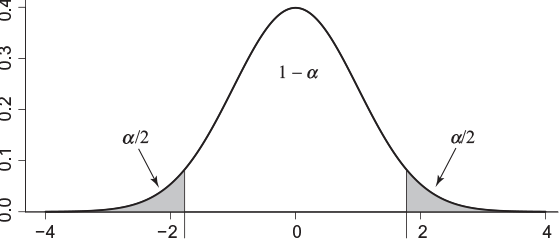
\includegraphics[keepaspectratio]{figs/7-twosided.png}}

\subsubsection{Rejection Region}

For two-sided tests with a significance level \(\alpha\), we need to
account for rejection regions on either side of the mean dictated by the
null hypothesis. Since the standard normal distribution is symmetric
about zero, the rejection region is defined by

\[
z < z_{\alpha/2}~OR~ z > z_{1-\alpha/2}
\] \#\#\# p-value

The p-value can be calculated using the following equation:

\[
P(Z < -|z|) + P(Z>|z|)
\] where \(|z|\) is the absolute value of \(z\).

\subsection{\texorpdfstring{Hypothesis Testing in
\texttt{R}}{Hypothesis Testing in R}}\label{hypothesis-testing-in-r}

We can use \texttt{pnorm(z)} to calculate the corresponding
probabilities after calculating the z-statistic. The arguments/options
for the \texttt{pnorm} function varies for the different alternative
hypotheses.

\subsection{Example}\label{example-3}

Suppose we have a sample of BMI levels for 200 adults. We assume the
population BMI levels are normally distributed with mean \(\mu\) and a
standard deviation of 5.0.

\subsubsection{Question}

Suppose the sample mean of the 200 adults was \(\bar{x}=22.9\). Test
whether the population BMI is equal to 23.5 against the alternative that
it is not 23.5. Use a significance level \(\alpha=0.05\)

\subsubsection{Answer 1 (p-value)}

The parameter of interest is the population average BMI. The null and
alternative hypotheses are as follows:

\[
H_0: \mu = 23.5; H_a: \mu \neq 23.5
\]

We first calculate the z-score, i.e.~the standardized statistic

\begin{Shaded}
\begin{Highlighting}[]
\NormalTok{xbar }\OtherTok{\textless{}{-}} \FloatTok{22.9}
\NormalTok{mu\_null }\OtherTok{\textless{}{-}} \FloatTok{23.5}
\NormalTok{stdev }\OtherTok{\textless{}{-}} \DecValTok{5}
\NormalTok{sampsize }\OtherTok{\textless{}{-}} \DecValTok{200}

\NormalTok{z }\OtherTok{\textless{}{-}}\NormalTok{ (xbar}\SpecialCharTok{{-}}\NormalTok{mu\_null)}\SpecialCharTok{/}\NormalTok{(stdev}\SpecialCharTok{/}\FunctionTok{sqrt}\NormalTok{(sampsize))}
\NormalTok{z}
\end{Highlighting}
\end{Shaded}

\begin{verbatim}
[1] -1.697056
\end{verbatim}

To calculate the p-value, we use \texttt{pnorm}. We can use
\texttt{abs(z)} to get the absolute value of \texttt{z}.

\begin{Shaded}
\begin{Highlighting}[]
\NormalTok{pval }\OtherTok{\textless{}{-}} \FunctionTok{pnorm}\NormalTok{(}\SpecialCharTok{{-}}\FunctionTok{abs}\NormalTok{(z)) }\SpecialCharTok{+} \FunctionTok{pnorm}\NormalTok{(}\FunctionTok{abs}\NormalTok{(z),}\AttributeTok{lower.tail=}\NormalTok{F)}
\NormalTok{pval}
\end{Highlighting}
\end{Shaded}

\begin{verbatim}
[1] 0.08968602
\end{verbatim}

The p-value is 0.09. The p-value is higher than the significance level,
which means we \textbf{fail to reject} the null hypothesis.

\subsubsection{Rejection Region}

To calculate the rejection region, we need \$ z \textless{}
z\_\{\alpha/2\}\textsubscript{OR} z \textgreater{} z\_\{1-\alpha/2\}\$.

The critical regions are then calculated as:

\begin{Shaded}
\begin{Highlighting}[]
\CommentTok{\# limit 1}
\NormalTok{alpha}\OtherTok{=}\FloatTok{0.05}
\FunctionTok{qnorm}\NormalTok{(}\FloatTok{0.05}\SpecialCharTok{/}\DecValTok{2}\NormalTok{)}
\end{Highlighting}
\end{Shaded}

\begin{verbatim}
[1] -1.959964
\end{verbatim}

\begin{Shaded}
\begin{Highlighting}[]
\CommentTok{\# limit 2}

\FunctionTok{qnorm}\NormalTok{(}\DecValTok{1}\SpecialCharTok{{-}}\NormalTok{alpha}\SpecialCharTok{/}\DecValTok{2}\NormalTok{)}
\end{Highlighting}
\end{Shaded}

\begin{verbatim}
[1] 1.959964
\end{verbatim}

The rejection region is then z \textless{} -1.959964 OR z \textgreater{}
1.959964Since z=-1.6970563 is not part of the rejection region, then we
fail to reject \(H_0\). We have insufficient evidence that the
population BMI is not equal to 23.5.

\subsubsection{Note}

\begin{tcolorbox}[enhanced jigsaw, bottomtitle=1mm, colback=white, opacityback=0, leftrule=.75mm, opacitybacktitle=0.6, coltitle=black, left=2mm, colframe=quarto-callout-note-color-frame, toptitle=1mm, colbacktitle=quarto-callout-note-color!10!white, titlerule=0mm, title=\textcolor{quarto-callout-note-color}{\faInfo}\hspace{0.5em}{Note}, arc=.35mm, rightrule=.15mm, breakable, bottomrule=.15mm, toprule=.15mm]

From here on out, we will use p-values to inform our decision about the
null hypothesis. Even though we are using p-values for hypothesis
testing, we must consider the fact that rejection regions and p-values
are inherently addressing different concepts.

\end{tcolorbox}

\subsection{Exercise}\label{exercise-1}

The scores of the Wechsler Adult Intelligence Scale are normally
distributed with a standard deviation of 15.

\subsubsection{Question}

Suppose an organization claims that the average IQ of their members are
above 131. A random sample of 40 members had an average Wechsler IQ
Score of 133.5. Use hypothesis testing to test the organization's claim.
Assume the sample size is negligible compared to the total membership of
the organization. Use a significant level \(\alpha = 0.05\).

\subsubsection{Answer}

The parameter of interest \(\mu\) is the population average IQ of the
organization. Our hypotheses are:

\[
H_0: \mu = 131; H_a: \mu > 131
\]

Calculating our test statistic \(z\),

\begin{Shaded}
\begin{Highlighting}[]
\NormalTok{xbar }\OtherTok{\textless{}{-}} \FloatTok{133.5}
\NormalTok{mu\_null }\OtherTok{\textless{}{-}} \DecValTok{131}
\NormalTok{stdev }\OtherTok{\textless{}{-}} \DecValTok{15}
\NormalTok{sampsize }\OtherTok{\textless{}{-}} \DecValTok{40}

\NormalTok{z }\OtherTok{\textless{}{-}}\NormalTok{ (xbar}\SpecialCharTok{{-}}\NormalTok{mu\_null)}\SpecialCharTok{/}\NormalTok{(stdev}\SpecialCharTok{/}\FunctionTok{sqrt}\NormalTok{(sampsize))}
\NormalTok{z}
\end{Highlighting}
\end{Shaded}

\begin{verbatim}
[1] 1.054093
\end{verbatim}

The resulting p-value for this one-sided test is: \(P(Z > z)\).

\begin{Shaded}
\begin{Highlighting}[]
\FunctionTok{pnorm}\NormalTok{(z,}\AttributeTok{lower.tail=}\NormalTok{F)}
\end{Highlighting}
\end{Shaded}

\begin{verbatim}
[1] 0.1459203
\end{verbatim}

The resulting p-value 0.15 is greater than the significance level of
0.05. Hence, we fail to reject the null hypothesis. We have insufficient
evidence that the population average Wechsler IQ scores of the
organization is above 131.

\subsection{Hypothesis Test: Single Mean, Unknown
Variance}\label{hypothesis-test-single-mean-unknown-variance}

When the population variance is unknown, we can use the
\(t-distribution\) to define our test statistic.

\begin{tcolorbox}[enhanced jigsaw, bottomtitle=1mm, colback=white, opacityback=0, leftrule=.75mm, opacitybacktitle=0.6, coltitle=black, left=2mm, colframe=quarto-callout-note-color-frame, toptitle=1mm, colbacktitle=quarto-callout-note-color!10!white, titlerule=0mm, title=\textcolor{quarto-callout-note-color}{\faInfo}\hspace{0.5em}{Note}, arc=.35mm, rightrule=.15mm, breakable, bottomrule=.15mm, toprule=.15mm]

Recall Chapter 6: We can substitute the sample variance for the
population variance and use the t-distribution instead of the standard
normal distribution to account for the additional variability due to the
variance estimation.

\end{tcolorbox}

If we are interested in testing the null hypothesis \(H_0: \mu=\mu_0\),
the alternative hypothesis can be one of the following:

\begin{itemize}
\tightlist
\item
  One-sided hypotheses: \(H_a: \mu < \mu_0\) or \(H_a: \mu > \mu_0\).
\item
  Two-sided hypotheses: \(H_a: \mu \neq \mu_0\)
\end{itemize}

The problem dictates which alternative is appropriate.

\subsection{Test Statistic}\label{test-statistic-2}

Recall that if \(\mu=\mu_0\) and the sample has a mean \(\bar{x}\),
variance \(s\), and size \(n\), then the following statistic, \(t\),
follows a t-distribution.

\[
t = \frac{\bar{X}-\mu_0}{s/\sqrt{n}}
\]

The statistic \(t\) follows a t-distribution with \(df=n-1\) degrees of
freedom.

\subsection{\texorpdfstring{Hypothesis Test:
\texttt{R}}{Hypothesis Test: R}}\label{hypothesis-test-r}

The test for a single mean and unknown variance is also known as the
\emph{one-sample t-test}. Here are the different ways to implement this
test in \texttt{R}.

\subsubsection{Given Statistics}

If we are given the mean, sample size, and standard deviation/variance,
we can calculate the t-statistic manually like we did for the
z-statistic for the case of known variance. We use the \texttt{pt()}
function to calculate the p-value.

\subsubsection{Given Data Set}

If we are provided a data set, we can use the
\texttt{t.test(vector,mu=mu\_null,alternative)} function in \texttt{R}.

\begin{tcolorbox}[enhanced jigsaw, bottomtitle=1mm, colback=white, opacityback=0, leftrule=.75mm, opacitybacktitle=0.6, coltitle=black, left=2mm, colframe=quarto-callout-important-color-frame, toptitle=1mm, colbacktitle=quarto-callout-important-color!10!white, titlerule=0mm, title=\textcolor{quarto-callout-important-color}{\faExclamation}\hspace{0.5em}{Important}, arc=.35mm, rightrule=.15mm, breakable, bottomrule=.15mm, toprule=.15mm]

\begin{itemize}
\tightlist
\item
  The \texttt{vector} includes the data that we want to use the t-test
  on.
\item
  The \texttt{mu\_null} placeholder is the mean according to the null
  hypothesis.
\item
  \texttt{alternative} can be \texttt{"less"} or \texttt{"greater"} for
  one-sided tests and \texttt{two.sided} for two-sided tests.
\end{itemize}

\end{tcolorbox}

\subsection{Example: Statistics}\label{example-statistics}

Suppose the recommendation for boys of a certain age is to consume at
least 1,200 calories per day. A dietary recall measure revealed that the
daily caloric intake for a random sample of 30 boys from the school
district who receive free lunches is 1100 and a standard deviation of
200 calories.

\subsubsection{Question}

Do we have sufficient evidence that the true mean daily caloric intake
for boys who receive free lunches from the school district is lower than
the recommended amount? Use a significance level of 0.05.

\subsubsection{Answer}

The parameter of interest is the true mean daily caloric intake for boys
who receive free lunches from the school district. The hypotheses are:

\[
H_0: \mu = 1200; H_a: \mu < 1200
\]

The summary statistics are provided, hence we need to calculate the
t-statistic manually.

\begin{Shaded}
\begin{Highlighting}[]
\NormalTok{xbar }\OtherTok{\textless{}{-}} \DecValTok{1100}
\NormalTok{mu\_null }\OtherTok{\textless{}{-}} \DecValTok{1200}
\NormalTok{sdsamp }\OtherTok{\textless{}{-}} \DecValTok{200}
\NormalTok{sampsize }\OtherTok{\textless{}{-}} \DecValTok{30}

\NormalTok{t}\OtherTok{\textless{}{-}}\NormalTok{ (xbar}\SpecialCharTok{{-}}\NormalTok{mu\_null)}\SpecialCharTok{/}\NormalTok{(sdsamp}\SpecialCharTok{/}\FunctionTok{sqrt}\NormalTok{(sampsize))}
\NormalTok{t}
\end{Highlighting}
\end{Shaded}

\begin{verbatim}
[1] -2.738613
\end{verbatim}

The t-statistic is -2.739. To calculate the p-value,

\begin{Shaded}
\begin{Highlighting}[]
\NormalTok{df }\OtherTok{\textless{}{-}}\NormalTok{ sampsize }\SpecialCharTok{{-}} \DecValTok{1}
\FunctionTok{dt}\NormalTok{(t,}\AttributeTok{df=}\NormalTok{df)}
\end{Highlighting}
\end{Shaded}

\begin{verbatim}
[1] 0.01255289
\end{verbatim}

The p-value is 0.01, which is less than \(\alpha\). We reject the null
hypothesis and conclude that there is sufficient evidence that the true
mean daily caloric intake for boys who receive free lunches from the
school district is lower than the recommended amount of 1,200 calories.

\subsection{Example: Data Set}\label{example-data-set}

The data set \texttt{Salaries} in the package \texttt{carData} includes
the The 2008-09 nine-month academic salary for Assistant Professors,
Associate Professors and Professors in a college in the U.S.

\subsubsection{Question}

Using the following code, we can isolate the salaries of the Assistant
Professors.

\begin{Shaded}
\begin{Highlighting}[]
\FunctionTok{library}\NormalTok{(carData)}
\NormalTok{asstprof }\OtherTok{\textless{}{-}} \FunctionTok{filter}\NormalTok{(Salaries, rank}\SpecialCharTok{==}\StringTok{"AsstProf"}\NormalTok{)}
\end{Highlighting}
\end{Shaded}

Do we have sufficient evidence that the average salary of the Assistant
Professors are above \$ 75,000? Use a significance level of 0.01.

\subsubsection{Answer}

The parameter of interest is the true average salary of the Assistant
Professors in a college in the U.S. The hypotheses are:

\[
H_0: \mu=75,000; H_a: \mu > 75,000
\]

We can use the \texttt{t.test()} function to implement the one-sample
t-test.

\begin{Shaded}
\begin{Highlighting}[]
\NormalTok{ttest }\OtherTok{\textless{}{-}} \FunctionTok{t.test}\NormalTok{(Salaries}\SpecialCharTok{$}\NormalTok{salary,}
       \AttributeTok{mu=}\DecValTok{75000}\NormalTok{,}
       \AttributeTok{alternative=}\StringTok{"greater"}\NormalTok{)}

\NormalTok{ttest}
\end{Highlighting}
\end{Shaded}

\begin{verbatim}

    One Sample t-test

data:  Salaries$salary
t = 25.462, df = 396, p-value < 2.2e-16
alternative hypothesis: true mean is greater than 75000
95 percent confidence interval:
 111200.1      Inf
sample estimates:
mean of x 
 113706.5 
\end{verbatim}

The test statistic is 25.462 with degrees of freedom df= 396. The
p-value is \texttt{\textless{}2.2e-16} which translates to a value lower
than \(2.2 \times 10^{-16}\). This is definitely lower than the
significance level of 0.01, hence we reject the null hypothesis. We have
sufficient evidence to support the claim that the average salary of the
Assistant Professors are above \$ 75,000.

\subsection{Exercise}\label{exercise-2}

Consider the data set \texttt{SleepHealthData.csv}.

\subsubsection{Question}

Test the hypothesis that the average sleep duration for the population
this sample represents is not equal to 7.5 hours. Use a significance
level of 0.05.

\begin{Shaded}
\begin{Highlighting}[]
\NormalTok{sleep }\OtherTok{\textless{}{-}} \FunctionTok{read.csv}\NormalTok{(}\StringTok{"SleepHealthData.csv"}\NormalTok{)}
\end{Highlighting}
\end{Shaded}

\subsubsection{Answer}

The parameter of interest is the population average sleep duration. The
hypotheses are:

\[
H_0: \mu=7; H_a: \mu \neq 7
\]

\begin{Shaded}
\begin{Highlighting}[]
\NormalTok{ttest }\OtherTok{\textless{}{-}} \FunctionTok{t.test}\NormalTok{(sleep}\SpecialCharTok{$}\NormalTok{sleep\_duration,}
       \AttributeTok{mu=}\DecValTok{7}\NormalTok{,}
       \AttributeTok{alternative=}\StringTok{"two.sided"}\NormalTok{)}

\NormalTok{ttest}
\end{Highlighting}
\end{Shaded}

\begin{verbatim}

    One Sample t-test

data:  sleep$sleep_duration
t = 3.2104, df = 373, p-value = 0.00144
alternative hypothesis: true mean is not equal to 7
95 percent confidence interval:
 7.051185 7.212986
sample estimates:
mean of x 
 7.132086 
\end{verbatim}

The test statistic is 3.2104 with degrees of freedom df= 373. The
p-value is 0.0014. This is definitely lower than the significance level
of 0.05, hence we reject the null hypothesis. We have sufficient
evidence that the population average sleep duration is not equal to 7.

\subsection{Hypothesis Test: Difference of Two Means (Independent
Groups)}\label{hypothesis-test-difference-of-two-means-independent-groups}

Often, we are interested in comparing two independent groups.

\begin{tcolorbox}[enhanced jigsaw, bottomtitle=1mm, colback=white, opacityback=0, leftrule=.75mm, opacitybacktitle=0.6, coltitle=black, left=2mm, colframe=quarto-callout-note-color-frame, toptitle=1mm, colbacktitle=quarto-callout-note-color!10!white, titlerule=0mm, title=\textcolor{quarto-callout-note-color}{\faInfo}\hspace{0.5em}{Note}, arc=.35mm, rightrule=.15mm, breakable, bottomrule=.15mm, toprule=.15mm]

Recall Chapters 5 and 6: To compare independent groups using a
continuous variable response, we investigate the difference between the
two groups. Examples of independent group comparisons include treatment
vs.~placebo, Location 1 vs.~Location 2, Male vs.~Female, Low vs.~High
SES.

\end{tcolorbox}

We are interested in testing the null hypothesis
\(H_0: \mu_1-\mu_2=\delta\). Most often, we use the null hypothesis of
equality where \(\delta=0\). The alternative hypothesis can be one of
the following:

\begin{itemize}
\tightlist
\item
  One-sided hypotheses: \(H_a: \mu_1-\mu_2 < \delta\) or
  \(H_a: \mu_1-\mu_2 > \delta\).
\item
  Two-sided hypotheses: \(H_a: \mu_1-\mu_2 \neq \delta\)
\end{itemize}

The problem dictates which alternative is appropriate as well as the
value of \(\delta\) (typically \(\delta=0\)).

\begin{tcolorbox}[enhanced jigsaw, bottomtitle=1mm, colback=white, opacityback=0, leftrule=.75mm, opacitybacktitle=0.6, coltitle=black, left=2mm, colframe=quarto-callout-important-color-frame, toptitle=1mm, colbacktitle=quarto-callout-important-color!10!white, titlerule=0mm, title=\textcolor{quarto-callout-important-color}{\faExclamation}\hspace{0.5em}{Important}, arc=.35mm, rightrule=.15mm, breakable, bottomrule=.15mm, toprule=.15mm]

The test comparing means of two independent groups is often referred to
as the two-sample t-test.

\end{tcolorbox}

\subsection{Test Statistic: Equal/Unequal
Variances}\label{test-statistic-equalunequal-variances}

The population variances are typically unknown, hence we use the
t-distribution for our test statistic.

\begin{tcolorbox}[enhanced jigsaw, bottomtitle=1mm, colback=white, opacityback=0, leftrule=.75mm, opacitybacktitle=0.6, coltitle=black, left=2mm, colframe=quarto-callout-warning-color-frame, toptitle=1mm, colbacktitle=quarto-callout-warning-color!10!white, titlerule=0mm, title=\textcolor{quarto-callout-warning-color}{\faExclamationTriangle}\hspace{0.5em}{Warning}, arc=.35mm, rightrule=.15mm, breakable, bottomrule=.15mm, toprule=.15mm]

Recall Chapter 6: Since we will be estimating the population variances
with sample variances, it is important to note whether we are assuming
equal or unequal population variances in defining the t-distribution for
our test statistic.

\end{tcolorbox}

\subsection{Test Statistic: Equal
Variances}\label{test-statistic-equal-variances}

Recall Chapter 6: or samples from two independent populations with equal
population variances, we use a pooled variance estimate, \(s_p^2\), for
the equal population variances.

\[
s_p^2 = \frac{(n_1-1)s_1^2 + (n_2-1)s_2^2}{n_1 + n_2 - 2}
\]

The t-statistic can then be calculated as

\[
t = \frac{(\bar{x}_1-\bar{x}_2) - (\mu_1-\mu_2)}{\sqrt{s_p^2\left(\frac{1}{n_1} + \frac{1}{n_2}\right)}}
\]

where \(\bar{x}_1\) and \(\bar{x}_2\) are the respective sample means
from Groups 1 and 2, \(s_p^2\) is the pooled variance, \(n_1\) and
\(n_2\) are the respective sample sizes from Groups 1 and 2. The
t-statistic follows a t-distribution with degrees of freedom
\(df=n_1 + n_2 - 2\).

\subsection{Test Statistic: Unequal
Variances}\label{test-statistic-unequal-variances}

Recall Chapter 6: For samples from two independent populations with
unequal population variances, we use tje \textbf{Welch-Satterthwaite}
procedure to construct this confidence interval such that the
\(100(1-\alpha)\)\% confidence interval is given by:

\[
t=\frac{(\bar{x}_1-\bar{x}_2) - (\mu_1-\mu_2)}{\sqrt{\left(\frac{s_1^2}{n_1} + \frac{s_2^2}{n_2}\right)}}
\]

where the degrees of freedom is provided by the Satterthwaite
approximation

\[
df = \frac{(s_1^2/n_1 + s_2^2/n_2)^2}{\left(\frac{s_1^2}{n_1}\right)^2/(n_1-1) + \left(\frac{s_2^2}{n_2}\right)^2/(n_2-1)}
\]

\subsection{\texorpdfstring{Hypothesis Testing:
\texttt{R}}{Hypothesis Testing: R}}\label{hypothesis-testing-r}

The function \texttt{t.test()} can be used to implement a two-sample
t-test. There are multiple ways to express the t-test using this
function in \texttt{R}.

\subsubsection{Column Grouping}

Suppose your data is assigned to the data frame \texttt{df} and the
measurements from the samples you want to compare are in different
columns: \texttt{col1} and \texttt{col2}. Suppose you have a null
hypothesis of equality, have a two-sided alternative, and assume equal
population variances. Then the t-test function can be coded as:

\begin{Shaded}
\begin{Highlighting}[]
\FunctionTok{t.test}\NormalTok{(}\AttributeTok{x=}\NormalTok{df}\SpecialCharTok{$}\NormalTok{col1,}
       \AttributeTok{y=}\NormalTok{df}\SpecialCharTok{$}\NormalTok{col2,}
       \AttributeTok{alternative=}\StringTok{"two.sided"}\NormalTok{,}
       \AttributeTok{mu=}\DecValTok{0}\NormalTok{,}
       \AttributeTok{var.equal=}\ConstantTok{TRUE}
\NormalTok{       )}
\end{Highlighting}
\end{Shaded}

\subsubsection{Variable Grouping}

Suppose your data is assigned to the data frame \texttt{df}, the
response measurements from the samples are in one column
\texttt{response}, and the groups are defined by a variable
\texttt{group}. Suppose you have a null hypothesis of equality, have a
two-sided alternative, and assume \emph{unequal} population variances.
We have to use the \textbf{formula} syntax in defining the groups. The
t-test function can be coded as:

\begin{Shaded}
\begin{Highlighting}[]
\FunctionTok{t.test}\NormalTok{(response}\SpecialCharTok{\textasciitilde{}}\NormalTok{group,}
       \AttributeTok{data=}\NormalTok{df,}
       \AttributeTok{alternative=}\StringTok{"two.sided"}\NormalTok{,}
       \AttributeTok{mu=}\DecValTok{0}\NormalTok{,}
       \AttributeTok{var.equal=}\ConstantTok{FALSE}
\NormalTok{       )}
\end{Highlighting}
\end{Shaded}

\begin{tcolorbox}[enhanced jigsaw, bottomtitle=1mm, colback=white, opacityback=0, leftrule=.75mm, opacitybacktitle=0.6, coltitle=black, left=2mm, colframe=quarto-callout-important-color-frame, toptitle=1mm, colbacktitle=quarto-callout-important-color!10!white, titlerule=0mm, title=\textcolor{quarto-callout-important-color}{\faExclamation}\hspace{0.5em}{Important}, arc=.35mm, rightrule=.15mm, breakable, bottomrule=.15mm, toprule=.15mm]

If the grouping variable is NOT a factor, the groups in the parameter of
interest \(\mu_1-\mu_2\) will be assigned in alphabetical order. If the
grouping variable is a factor, it will follow the order set in the
factor.

\end{tcolorbox}

\subsection{Example}\label{example-4}

Consider the sleep health data set from \texttt{SleepHealthData.csv}.

\subsubsection{Question}

Perform a hypothesis test to determine if there is any statistically
discernible difference between the average sleep duration of males and
females. Assume equal variances and a significance level of 0.05.

\subsubsection{Answer}

The parameter of interest is the \textbf{true difference} in average
sleep duration of males and females (\(\mu_f-\mu_m\)). The hypotheses
should be:

\[
H_0: \mu_f - \mu_m = 0; H_a: \mu_f - \mu_m \neq 0
\] The alternative is two-sided because we did not specify a direction
of the difference between the two groups.

The groups are defined by the variable \texttt{gender} and the response
variable is defined by the variable \texttt{sleep\_duration}. The t-test
can be implemented using the following code:

\begin{Shaded}
\begin{Highlighting}[]
\CommentTok{\# Set working directory where the Sleep Health Data is saved.}
\NormalTok{sleep }\OtherTok{\textless{}{-}} \FunctionTok{read.csv}\NormalTok{(}\StringTok{"SleepHealthData.csv"}\NormalTok{)}
\NormalTok{ttest }\OtherTok{\textless{}{-}} \FunctionTok{t.test}\NormalTok{(sleep\_duration}\SpecialCharTok{\textasciitilde{}}\NormalTok{gender,}
                \AttributeTok{data=}\NormalTok{sleep,}
                \AttributeTok{mu=}\DecValTok{0}\NormalTok{,}
                \AttributeTok{alternative=}\StringTok{"two.sided"}\NormalTok{,}
                \AttributeTok{var.equal=}\ConstantTok{TRUE}\NormalTok{)}

\NormalTok{ttest}
\end{Highlighting}
\end{Shaded}

\begin{verbatim}

    Two Sample t-test

data:  sleep_duration by gender
t = 2.3624, df = 372, p-value = 0.01867
alternative hypothesis: true difference in means between group Female and group Male is not equal to 0
95 percent confidence interval:
 0.03239537 0.35404821
sample estimates:
mean in group Female   mean in group Male 
            7.229730             7.036508 
\end{verbatim}

The p-value is 0.0187, which is lower than the set significance level of
0.05. We reject the null hypothesis. We have sufficient evidence that
the true difference in average sleep duration between females and males
is non-zero.

\subsection{Example}\label{example-5}

The data set \texttt{hflashes\_subset.csv} contains the baseline FSH
measurements of 50 randomly sampled participants the following groups:
those who reported hot flashes and those who did not.

\subsubsection{Question}

Is there a discernible difference between the average FSH levels of
those who reported hot flashes and those who did not? Use a significance
level of 0.01. Assume unequal population variances.

\subsubsection{Answer}

The parameter of interest is the \textbf{true difference} in average FSH
levels between those who experienced hot flashes and who did not. The
hypotheses should be:

\[
H_0: \mu_h - \mu_n = 0; H_a: \mu_h - \mu_n \neq 0
\] The alternative is two-sided because we did not specify a direction
of the difference between the two groups.

The groups are defined by the columns: \texttt{YesHotFlash} and
\texttt{NoHotFlash}. The t-test can be implemented using the following
code:

\begin{Shaded}
\begin{Highlighting}[]
\CommentTok{\# Set working directory where the Sleep Health Data is saved.}
\NormalTok{fsh }\OtherTok{\textless{}{-}} \FunctionTok{read.csv}\NormalTok{(}\StringTok{"hflashes\_subset.csv"}\NormalTok{)}
\NormalTok{ttest }\OtherTok{\textless{}{-}} \FunctionTok{t.test}\NormalTok{(}\AttributeTok{x=}\NormalTok{fsh}\SpecialCharTok{$}\NormalTok{YesHotFlash,}
                \AttributeTok{y=}\NormalTok{fsh}\SpecialCharTok{$}\NormalTok{NoHotFlash,}
                \AttributeTok{mu=}\DecValTok{0}\NormalTok{,}
                \AttributeTok{alternative=}\StringTok{"two.sided"}\NormalTok{,}
                \AttributeTok{var.equal=}\ConstantTok{FALSE}\NormalTok{)}

\NormalTok{ttest}
\end{Highlighting}
\end{Shaded}

\begin{verbatim}

    Welch Two Sample t-test

data:  fsh$YesHotFlash and fsh$NoHotFlash
t = 0.040448, df = 97.999, p-value = 0.9678
alternative hypothesis: true difference in means is not equal to 0
95 percent confidence interval:
 -2.085887  2.172687
sample estimates:
mean of x mean of y 
   9.6598    9.6164 
\end{verbatim}

The p-value is 0.9678, which is higher than the set significance level
of 0.01. We fail to reject the null hypothesis. We have insufficient
evidence that the true difference in average fsh levels between those
who experience hot flashes and who did not is non-zero.

\subsection{Exercise}\label{exercise-3}

Consider the sleep health data set from \texttt{SleepHealthData.csv}.

\subsubsection{Question}

Perform a hypothesis test to determine if the average heart rate of
males is higher than that of females. Assume equal variances and a
significance level of 0.05.

\begin{tcolorbox}[enhanced jigsaw, bottomtitle=1mm, colback=white, opacityback=0, leftrule=.75mm, opacitybacktitle=0.6, coltitle=black, left=2mm, colframe=quarto-callout-warning-color-frame, toptitle=1mm, colbacktitle=quarto-callout-warning-color!10!white, titlerule=0mm, title=\textcolor{quarto-callout-warning-color}{\faExclamationTriangle}\hspace{0.5em}{Warning}, arc=.35mm, rightrule=.15mm, breakable, bottomrule=.15mm, toprule=.15mm]

The group levels will follow \emph{alphabetical order}, which means
group 1 will be set as the female group.

\end{tcolorbox}

\subsubsection{Answer}

The parameter of interest is the \textbf{true difference} in average
heart rate between females and males (\(\mu_f-\mu_m\)). The hypotheses
should be:

\[
H_0: \mu_f - \mu_m = 0; H_a: \mu_f - \mu_m < 0
\] The alternative is one-sided, ``less'', because we specified the
direction where males have a higher average heart rate than females.

The groups are defined by the variable \texttt{gender} and the response
variable is defined by the variable \texttt{heart\_rate}. The t-test can
be implemented using the following code:

\begin{Shaded}
\begin{Highlighting}[]
\CommentTok{\# Set working directory where the Sleep Health Data is saved.}
\NormalTok{sleep }\OtherTok{\textless{}{-}} \FunctionTok{read.csv}\NormalTok{(}\StringTok{"SleepHealthData.csv"}\NormalTok{) }\CommentTok{\# if not already loaded}
\NormalTok{ttest }\OtherTok{\textless{}{-}} \FunctionTok{t.test}\NormalTok{(heart\_rate}\SpecialCharTok{\textasciitilde{}}\NormalTok{gender,}
                \AttributeTok{data=}\NormalTok{sleep,}
                \AttributeTok{mu=}\DecValTok{0}\NormalTok{,}
                \AttributeTok{alternative=}\StringTok{"less"}\NormalTok{,}
                \AttributeTok{var.equal=}\ConstantTok{TRUE}\NormalTok{)}

\NormalTok{ttest}
\end{Highlighting}
\end{Shaded}

\begin{verbatim}

    Two Sample t-test

data:  heart_rate by gender
t = -4.2897, df = 372, p-value = 1.142e-05
alternative hypothesis: true difference in means between group Female and group Male is less than 0
95 percent confidence interval:
      -Inf -1.104046
sample estimates:
mean in group Female   mean in group Male 
            69.25946             71.05291 
\end{verbatim}

The p-value is 0.000011, which is lower than the set significance level
of 0.05. We reject the null hypothesis. We have sufficient evidence that
the true difference in average heart rate between females and males is
less than zero. Or we can say: We have sufficient evidence that the
average heart rate of males is higher than that of females in the
population this sample represents.

\subsection{Hypothesis Testing: Paired
Means}\label{hypothesis-testing-paired-means}

There are times when two sets of measurements cannot be treated as
independent groups. Consider the following example: The table below
shows the pre- and post-test scores of five students after going through
a newly developed statistics course.

\begin{longtable}[]{@{}lll@{}}
\toprule\noalign{}
Student ID & Pre-Test & Post-Test \\
\midrule\noalign{}
\endhead
\bottomrule\noalign{}
\endlastfoot
1 & 75 & 77 \\
2 & 62 & 64 \\
3 & 51 & 53 \\
4 & 55 & 57 \\
5 & 97 & 99 \\
\end{longtable}

\begin{tcolorbox}[enhanced jigsaw, bottomtitle=1mm, colback=white, opacityback=0, leftrule=.75mm, opacitybacktitle=0.6, coltitle=black, left=2mm, colframe=quarto-callout-note-color-frame, toptitle=1mm, colbacktitle=quarto-callout-note-color!10!white, titlerule=0mm, title=\textcolor{quarto-callout-note-color}{\faInfo}\hspace{0.5em}{Note}, arc=.35mm, rightrule=.15mm, breakable, bottomrule=.15mm, toprule=.15mm]

There is a lot of variability among the pre-test and post-test scores.
However, the \textbf{paired} differences show an increase of two points
for \textbf{all} students, showing no variability between students.

\end{tcolorbox}

\subsection{Paired Means}\label{paired-means}

For dependent means, the parameter of interest is the \textbf{true
average of the paired differences} which we will refer to as \(mu_d\).

\begin{tcolorbox}[enhanced jigsaw, bottomtitle=1mm, colback=white, opacityback=0, leftrule=.75mm, opacitybacktitle=0.6, coltitle=black, left=2mm, colframe=quarto-callout-note-color-frame, toptitle=1mm, colbacktitle=quarto-callout-note-color!10!white, titlerule=0mm, title=\textcolor{quarto-callout-note-color}{\faInfo}\hspace{0.5em}{Note}, arc=.35mm, rightrule=.15mm, breakable, bottomrule=.15mm, toprule=.15mm]

Paired measurements can come from repeated measures from the same unit
(Ex: pre- vs.~post-test for a single student) or from matched pairs (two
individuals with the same demographic and genetic background going
through a randomized controlled trial).

\end{tcolorbox}

We are interested in testing the null hypothesis \(H_0: \mu_d=d_0\).
Most often, we use the null hypothesis of equality where \(d_0=0\). The
alternative hypothesis can be one of the following:

\begin{itemize}
\tightlist
\item
  One-sided hypotheses: \(H_a: \mu_d< d_0\) or \(H_a: \mu_d> d_0\).
\item
  Two-sided hypotheses: \(H_a: \mu_d \neq d_0\)
\end{itemize}

The problem dictates which alternative is appropriate as well as the
value of \(d_0\) (typically \(d_0=0\) for the null hypothesis of
equality).

\subsection{Test Statistic}\label{test-statistic-3}

Recall that we do not know the population variance of the paired
differences, hence we need to use the t-distribution. if \(\mu_d=d_0\)
and the sample has a mean paired difference \(\bar{x}_d\), variance
\(s_d\), and number of paired observations \(n\), then the following
statistic, \(t\), follows a t-distribution.

\[
t = \frac{\bar{x}_d-d_0}{s_d/\sqrt{n}}
\]

The statistic \(t\) follows a t-distribution with \(df=n-1\) degrees of
freedom.

\subsection{\texorpdfstring{Hypothesis Test:
\texttt{R}}{Hypothesis Test: R}}\label{hypothesis-test-r-1}

The test for paired differences is also known as the \emph{paired
t-test}. Here are the different ways to implement this test in
\texttt{R}.

\subsubsection{Given Statistics}

If we are given the mean, sample size, and standard deviation/variance,
we can calculate the t-statistic manually like we did for the
z-statistic for the case of known variance. We use the \texttt{pt()}
function to calculate the p-value.

\subsubsection{Given Data Set}

Suppose your data is assigned to the data frame \texttt{df} and the
measurements from the samples you want to compare are in different
columns: \texttt{col1} and \texttt{col2}. Suppose you have a null
hypothesis \(H_0: \mu_d=d_0\), have a two-sided alternative, and assume
equal population variances. Then the t-test function can be coded as:

\begin{Shaded}
\begin{Highlighting}[]
\FunctionTok{t.test}\NormalTok{(}\AttributeTok{x=}\NormalTok{df}\SpecialCharTok{$}\NormalTok{col1,}
       \AttributeTok{y=}\NormalTok{df}\SpecialCharTok{$}\NormalTok{col2,}
       \AttributeTok{alternative=}\StringTok{"two.sided"}\NormalTok{,}
       \AttributeTok{mu=}\NormalTok{d\_0,}
       \AttributeTok{paired=}\ConstantTok{TRUE}
\NormalTok{       )}
\end{Highlighting}
\end{Shaded}

\begin{tcolorbox}[enhanced jigsaw, bottomtitle=1mm, colback=white, opacityback=0, leftrule=.75mm, opacitybacktitle=0.6, coltitle=black, left=2mm, colframe=quarto-callout-warning-color-frame, toptitle=1mm, colbacktitle=quarto-callout-warning-color!10!white, titlerule=0mm, title=\textcolor{quarto-callout-warning-color}{\faExclamationTriangle}\hspace{0.5em}{Warning}, arc=.35mm, rightrule=.15mm, breakable, bottomrule=.15mm, toprule=.15mm]

The formula syntax will not work for paired data. The paired variables
should be coded as two separate columns.

\end{tcolorbox}

\subsection{Example}\label{example-6}

The data set \texttt{anorexia} from the package \texttt{MASS} contains
weight change data for young female anorexia patients.

\begin{Shaded}
\begin{Highlighting}[]
\FunctionTok{library}\NormalTok{(MASS)}
\end{Highlighting}
\end{Shaded}

\begin{verbatim}

Attaching package: 'MASS'
\end{verbatim}

\begin{verbatim}
The following object is masked from 'package:dplyr':

    select
\end{verbatim}

\begin{Shaded}
\begin{Highlighting}[]
\FunctionTok{library}\NormalTok{(tidyverse)}
\FunctionTok{glimpse}\NormalTok{(anorexia)}
\end{Highlighting}
\end{Shaded}

\begin{verbatim}
Rows: 72
Columns: 3
$ Treat  <fct> Cont, Cont, Cont, Cont, Cont, Cont, Cont, Cont, Cont, Cont, Con~
$ Prewt  <dbl> 80.7, 89.4, 91.8, 74.0, 78.1, 88.3, 87.3, 75.1, 80.6, 78.4, 77.~
$ Postwt <dbl> 80.2, 80.1, 86.4, 86.3, 76.1, 78.1, 75.1, 86.7, 73.5, 84.6, 77.~
\end{verbatim}

\subsubsection{Question}

Perform a paired t-test to test whether there is a difference between
the preweight \texttt{prewt} and \texttt{postwt} for all patients,
disregarding the type of treatment. Use a significance level of 0.05.

\subsubsection{Answer}

The parameter of interest is the average paired difference in weight
before and after treatment, \(\mu_d\). The hypotheses are:

\[
H_0: \mu_d = 0; H_a: \mu_d \neq 0
\] We can use \texttt{t.test()} to perform the t-test.

\begin{Shaded}
\begin{Highlighting}[]
\NormalTok{ttest }\OtherTok{\textless{}{-}} \FunctionTok{t.test}\NormalTok{(}\AttributeTok{x=}\NormalTok{anorexia}\SpecialCharTok{$}\NormalTok{Postwt,}
       \AttributeTok{y=}\NormalTok{anorexia}\SpecialCharTok{$}\NormalTok{Prewt,}
       \AttributeTok{alternative=}\StringTok{"two.sided"}\NormalTok{,}
       \AttributeTok{mu=}\DecValTok{0}\NormalTok{,}
       \AttributeTok{paired=}\ConstantTok{TRUE}
\NormalTok{       )}
\NormalTok{ttest}
\end{Highlighting}
\end{Shaded}

\begin{verbatim}

    Paired t-test

data:  anorexia$Postwt and anorexia$Prewt
t = 2.9376, df = 71, p-value = 0.004458
alternative hypothesis: true mean difference is not equal to 0
95 percent confidence interval:
 0.8878354 4.6399424
sample estimates:
mean difference 
       2.763889 
\end{verbatim}

The p-value is 0.0045, which is lower than the set significance level of
0.05. We reject the null hypothesis. We have sufficient evidence that
the true average paired difference in weight pre- and post-treatment is
not zero.

\subsection{Exercise}\label{exercise-4}

The data set \texttt{ChickWeight.csv} contains 10 paired data
corresponding to weights of chicks in ounces, two from 10 families,
reared in confinement or on open range.

\begin{Shaded}
\begin{Highlighting}[]
\CommentTok{\# Remember to save ChickWeight to your working directory}
\NormalTok{chick }\OtherTok{\textless{}{-}} \FunctionTok{read.csv}\NormalTok{(}\StringTok{"ChickWeight.csv"}\NormalTok{)}
\FunctionTok{glimpse}\NormalTok{(chick)}
\end{Highlighting}
\end{Shaded}

\begin{verbatim}
Rows: 10
Columns: 3
$ Chicks      <chr> "C01", "C02", "C03", "C04", "C05", "C06", "C07", "C08", "C~
$ Confinement <int> 9, 17, 14, 13, 15, 10, 11, 13, 13, 15
$ OpenRange   <int> 8, 15, 11, 11, 9, 12, 11, 10, 9, 14
\end{verbatim}

\subsubsection{Question}

Suppose the farmer claims that the difference in weights between chicks
raised in confinement and those who were raised in open range is higher
than 1.5 ounces. Perform a hypothesis test that tests this claim. Use a
significance level of 0.05.

\subsubsection{Answer}

Note that the chicks were paired up with another chick from the same
family, hence we need to use a paired t-test. The parameter of interest
is the true average paired difference in weights of chicks raised in
confinement and open range. The hypotheses can be written as:

\[
H_0: \mu_d = 1.5; H_a: \mu_d > 1.5
\] Define the difference as \texttt{Confinement-OpenRange}. We can now
implement the t-test using the \texttt{t.test()} function.

\begin{Shaded}
\begin{Highlighting}[]
\NormalTok{ttest }\OtherTok{\textless{}{-}} \FunctionTok{t.test}\NormalTok{(}\AttributeTok{x=}\NormalTok{chick}\SpecialCharTok{$}\NormalTok{Confinement,}
       \AttributeTok{y=}\NormalTok{chick}\SpecialCharTok{$}\NormalTok{OpenRange,}
       \AttributeTok{alternative=}\StringTok{"greater"}\NormalTok{,}
       \AttributeTok{mu=}\FloatTok{1.5}\NormalTok{,}
       \AttributeTok{paired=}\ConstantTok{TRUE}
\NormalTok{       )}
\NormalTok{ttest}
\end{Highlighting}
\end{Shaded}

\begin{verbatim}

    Paired t-test

data:  chick$Confinement and chick$OpenRange
t = 0.7151, df = 9, p-value = 0.2463
alternative hypothesis: true mean difference is greater than 1.5
95 percent confidence interval:
 0.7182766       Inf
sample estimates:
mean difference 
              2 
\end{verbatim}

The p-value is 0.2463, which is higher than the set significance level
of 0.05. We fail reject the null hypothesis. We have insufficient
evidence that the true average paired difference in weight of chicks
raised in confinement and open range is higher than 1.5 ounces.

\subsection{Hypothesis Test: Single Population
Proportion}\label{hypothesis-test-single-population-proportion}

We can also perform hypothesis tests for a single proportion, \(\pi\).

We are interested in testing the null hypothesis \(H_0: \pi=\pi_0\). The
alternative hypothesis can be one of the following:

\begin{itemize}
\tightlist
\item
  One-sided hypotheses: \(H_a: \pi>\pi_0\) or \(H_a: \pi<\pi_0\).
\item
  Two-sided hypotheses: \(H_a: \pi \neq \pi_0\)
\end{itemize}

\subsection{Test Statistic}\label{test-statistic-4}

\begin{tcolorbox}[enhanced jigsaw, bottomtitle=1mm, colback=white, opacityback=0, leftrule=.75mm, opacitybacktitle=0.6, coltitle=black, left=2mm, colframe=quarto-callout-note-color-frame, toptitle=1mm, colbacktitle=quarto-callout-note-color!10!white, titlerule=0mm, title=\textcolor{quarto-callout-note-color}{\faInfo}\hspace{0.5em}{Note}, arc=.35mm, rightrule=.15mm, breakable, bottomrule=.15mm, toprule=.15mm]

Recall Chapter 6: When dealing with inference related to proportions,
the reliability coefficient we used was derived from the standard normal
distribution. In Chapter 7, we will use the standard normal distribution
to describe our test statistic: the z-statistic.

\end{tcolorbox}

For a sample proportion \(\hat{p}\) and sample size \(n\), the
z-statistic can be expressed as \[
z = \frac{\hat{p}-\pi_0}{\sqrt{\frac{\pi_0(1-\pi_0)}{n}}}.
\]

\subsection{\texorpdfstring{Hypothesis Testing:
\texttt{R}}{Hypothesis Testing: R}}\label{hypothesis-testing-r-1}

We can use \texttt{pnorm(z)} to calculate the corresponding
probabilities after calculating the z-statistic. The arguments/options
for the \texttt{pnorm} function varies for the different alternative
hypotheses. Similar to the hypothesis test for a single mean with known
variance, the p-values can be calculated as:

\begin{itemize}
\tightlist
\item
  \(H_a: \pi < \pi_0 \to P(Z < z)\)
\item
  \(H_a: \pi > \pi_0 \to P(Z > z)\)
\item
  \(H_a: \pi \neq \pi_0 \to P(Z < -|z|) + P(Z>|z|)\)
\end{itemize}

\subsection{Example}\label{example-7}

Suppose the health department claims that the vaccination rate for
shingles in older adults in the population is above 50\%. When a random
sample of elderly adults were asked about their vaccination status, 357
out of 700 reported to be vaccinated against shingles.

\subsubsection{Question}

Perform a hypothesis test to test the claim of the health department.
Use a significance level of 0.01.

\subsubsection{Answer}

The parameter of interest is the \textbf{true proportion of elderly
adults vaccinated against shingles}. The hypotheses are:

\[
H_0: \pi = 0.5; H_a: \pi > 0.5
\]

Our sample proportion is 357/700 with a sample size of 700. We can now
calculate the z-statistic

\begin{Shaded}
\begin{Highlighting}[]
\NormalTok{sampsize }\OtherTok{\textless{}{-}} \DecValTok{700}
\NormalTok{phat }\OtherTok{\textless{}{-}} \DecValTok{357}\SpecialCharTok{/}\NormalTok{sampsize}
\NormalTok{pi\_null }\OtherTok{\textless{}{-}} \FloatTok{0.5}
\NormalTok{se }\OtherTok{\textless{}{-}} \FunctionTok{sqrt}\NormalTok{(pi\_null}\SpecialCharTok{*}\NormalTok{(}\DecValTok{1}\SpecialCharTok{{-}}\NormalTok{pi\_null)}\SpecialCharTok{/}\NormalTok{sampsize)}

\NormalTok{z }\OtherTok{\textless{}{-}}\NormalTok{ (phat}\SpecialCharTok{{-}}\NormalTok{pi\_null)}\SpecialCharTok{/}\NormalTok{se}
\NormalTok{z}
\end{Highlighting}
\end{Shaded}

\begin{verbatim}
[1] 0.5291503
\end{verbatim}

The corresponding p-value should be calculated as P(Z \textgreater{}
0.5291503)

\begin{Shaded}
\begin{Highlighting}[]
\FunctionTok{pnorm}\NormalTok{(z,}\AttributeTok{lower.tail=}\NormalTok{F)}
\end{Highlighting}
\end{Shaded}

\begin{verbatim}
[1] 0.2983506
\end{verbatim}

The resulting p-value is 0.2983506, which is higher than the
significance level of 0.01. We fail to reject the null hypothesis. We
have insufficient evidence to claim that the true percentage of elderly
adults vaccinated against shingles in this population is higher than
50\%.

\subsection{Exercise}\label{exercise-5}

Consider the sleep health data \texttt{SleepHealthData.csv}

\begin{Shaded}
\begin{Highlighting}[]
\NormalTok{sleep }\OtherTok{\textless{}{-}} \FunctionTok{read.csv}\NormalTok{(}\StringTok{"SleepHealthData.csv"}\NormalTok{)}
\end{Highlighting}
\end{Shaded}

\subsubsection{Question}

Suppose the claim is that the prevalence rate of sleep apnea in this
population is lower than 25\%. Do we have evidence to support this
claim? Use a significance level of 0.10.

\subsubsection{Answer}

The parameter of interest is the \textbf{true proportion of the
population who have sleep apnea}. The hypotheses are:

\[
H_0: \pi = 0.25; H_a: \pi < 0.25
\]

We can calculate the sample proportion using the frequency table
provided by \texttt{freq()} from the \texttt{summarytools} package.

\begin{Shaded}
\begin{Highlighting}[]
\FunctionTok{library}\NormalTok{(summarytools)}
\end{Highlighting}
\end{Shaded}

\begin{verbatim}

Attaching package: 'summarytools'
\end{verbatim}

\begin{verbatim}
The following object is masked from 'package:tibble':

    view
\end{verbatim}

\begin{Shaded}
\begin{Highlighting}[]
\FunctionTok{freq}\NormalTok{(sleep}\SpecialCharTok{$}\NormalTok{sleep\_disorder)}
\end{Highlighting}
\end{Shaded}

\begin{verbatim}
Frequencies  
sleep$_disorder  
Type: Character  

                    Freq   % Valid   % Valid Cum.   % Total   % Total Cum.
----------------- ------ --------- -------------- --------- --------------
         Insomnia     77     20.59          20.59     20.59          20.59
             None    219     58.56          79.14     58.56          79.14
      Sleep Apnea     78     20.86         100.00     20.86         100.00
             <NA>      0                               0.00         100.00
            Total    374    100.00         100.00    100.00         100.00
\end{verbatim}

We can now calculate the z-statistic

\begin{Shaded}
\begin{Highlighting}[]
\NormalTok{sampsize }\OtherTok{\textless{}{-}} \DecValTok{374}
\NormalTok{phat }\OtherTok{\textless{}{-}} \DecValTok{78}\SpecialCharTok{/}\NormalTok{sampsize}
\NormalTok{pi\_null }\OtherTok{\textless{}{-}} \FloatTok{0.25}
\NormalTok{se }\OtherTok{\textless{}{-}} \FunctionTok{sqrt}\NormalTok{(pi\_null}\SpecialCharTok{*}\NormalTok{(}\DecValTok{1}\SpecialCharTok{{-}}\NormalTok{pi\_null)}\SpecialCharTok{/}\NormalTok{sampsize)}

\NormalTok{z }\OtherTok{\textless{}{-}}\NormalTok{ (phat}\SpecialCharTok{{-}}\NormalTok{pi\_null)}\SpecialCharTok{/}\NormalTok{se}
\NormalTok{z}
\end{Highlighting}
\end{Shaded}

\begin{verbatim}
[1] -1.850952
\end{verbatim}

The corresponding p-value should be calculated as P(Z \textless{}
-1.8509524)

\begin{Shaded}
\begin{Highlighting}[]
\FunctionTok{pnorm}\NormalTok{(z)}
\end{Highlighting}
\end{Shaded}

\begin{verbatim}
[1] 0.0320882
\end{verbatim}

The resulting p-value is 0.0320882, which is lower than the significance
level of 0.10. We reject the null hypothesis. We have sufficient
evidence to claim that the true prevalence rate of sleep apnea in this
population is lower than 25\%.

\subsection{Hypothesis Test: Difference of Two Population
Proportions}\label{hypothesis-test-difference-of-two-population-proportions}

We can also expand the hypothesis tests to compare proportions from two
populations using their difference, \(\pi_1 - \pi_2\).

We are interested in testing the null hypothesis of equality
\(H_0: \pi_1 - \pi_2=0\). The alternative hypothesis can be one of the
following:

\begin{itemize}
\tightlist
\item
  One-sided hypotheses: \(H_a: \pi_1 - \pi_2>0\) or
  \(H_a: \pi_1 - \pi_2<0\).
\item
  Two-sided hypotheses: \(H_a: \pi_1 - \pi_2\neq 0\)
\end{itemize}

\subsection{Test Statistic}\label{test-statistic-5}

When testing the null hypothesis \(H_0: \pi_1 - \pi_2=0\), the standard
error used in calculating the z-statistic involves the pooled proportion
\(\bar{p}\), given by:

\[
\bar{p} = \frac{x_1 + x_2}{n_1 + n_2} = \frac{n_1p_1 + n_2x_2}{n_1 + n_2}
\]

where the number of successes are \(x_1\) and \(x_2\), sample
proportions are \(\hat{p}_1\) and \(\hat{p}_2\), and sample sizes are
\(n_1\) and \(n_2\). The z-statistic can be calculated using the
following equation:

\[
z = \frac{\hat{p}_1 -\hat{p}_2}{\sqrt{\bar{p}(1-\bar{p})\left(\frac{1}{n_1} + \frac{1}{n_2}\right)}}.
\]

\subsection{Example}\label{example-8}

Consider the hotflash data set \texttt{hflashes.csv}. The variable
\texttt{f1a} has a value of 1 if the participant currently smokes and 0
otherwise.

\begin{Shaded}
\begin{Highlighting}[]
\NormalTok{hflashes }\OtherTok{\textless{}{-}} \FunctionTok{read.csv}\NormalTok{(}\StringTok{"datasets/hflashes.csv"}\NormalTok{)}
\FunctionTok{glimpse}\NormalTok{(hflashes)}
\end{Highlighting}
\end{Shaded}

\begin{verbatim}
Rows: 375
Columns: 14
$ pt       <int> 3, 6, 7, 8, 9, 10, 11, 12, 13, 14, 15, 16, 17, 19, 20, 23, 24~
$ ageg     <int> 2, 3, 1, 1, 2, 3, 2, 2, 2, 3, 2, 1, 1, 1, 1, 3, 2, 1, 1, 1, 2~
$ aagrp    <int> 0, 0, 0, 0, 0, 0, 0, 1, 0, 0, 1, 1, 0, 1, 1, 0, 0, 0, 0, 1, 0~
$ edu      <int> 1, 1, 1, 1, 1, 1, 1, 1, 1, 1, 1, 0, 1, 1, 1, 1, 0, 1, 1, 1, 1~
$ d1       <int> 0, 0, 0, 1, 0, 0, 0, 0, 1, 0, 1, 1, 1, 1, 0, 0, 0, 1, 0, 1, 0~
$ f1a      <int> 0, 0, 1, 0, 1, 0, 0, 1, 1, 0, 0, 1, 0, 0, 1, 1, 1, 0, 0, 0, 1~
$ pcs12    <dbl> 56.80537, 59.18338, 57.73952, 55.83575, 55.89324, NA, 55.5009~
$ hotflash <int> 0, 0, 0, 1, 0, 1, 0, 1, 1, 0, 1, 0, 0, 0, 0, 0, 0, 1, 0, 1, 0~
$ bmi30    <int> 0, 0, 0, 0, 0, 0, 1, 1, 0, 0, 1, 1, 0, 0, 0, 0, 0, 0, 0, 1, 0~
$ estra    <dbl> 106.710, 31.250, 13.410, 10.640, 24.060, 37.305, 26.320, 24.1~
$ fsh      <dbl> 3.005, 11.195, 14.545, 5.530, 9.780, 10.290, 7.960, 4.775, 7.~
$ lh       <dbl> 2.980, 5.760, 5.595, 2.260, 2.600, 3.395, 3.570, 2.095, 3.660~
$ testo    <dbl> 7.680, 11.930, 24.375, 8.280, 4.050, 8.275, 15.995, 12.340, 1~
$ dheas    <dbl> 61.225, 104.920, 117.450, 36.850, 11.165, 100.360, 76.780, 83~
\end{verbatim}

\subsubsection{Question}

Does this study provide sufficient evidence for us to conclude that
participants who smoke have a higher proportion of participants who
experience hot flashes compared to those who do not smoke? Use
\(\alpha=0.05\).

\subsubsection{Answer}

The parameter of interest is the \textbf{true difference in proportion
of participants who experience hot flashes between current and
nonsmokers.}. The hypotheses are:

\[
H_0: \pi_s-\pi_n = 0; H_a: \pi_s-\pi_n > 0
\] Calculating the proportions would be slightly more complicated with
two groups. We will use the \texttt{filter(data,condition)} function to
separate the smokers and the non-smokers based on the \texttt{f1a}
variable.

\begin{Shaded}
\begin{Highlighting}[]
\NormalTok{smokers }\OtherTok{\textless{}{-}} \FunctionTok{filter}\NormalTok{(hflashes,f1a}\SpecialCharTok{==}\DecValTok{1}\NormalTok{)}
\NormalTok{nonsmokers }\OtherTok{\textless{}{-}} \FunctionTok{filter}\NormalTok{(hflashes,f1a}\SpecialCharTok{==}\DecValTok{0}\NormalTok{)}

\FunctionTok{freq}\NormalTok{(smokers}\SpecialCharTok{$}\NormalTok{hotflash)}
\end{Highlighting}
\end{Shaded}

\begin{verbatim}
Frequencies  
smokers$hotflash  
Type: Integer  

              Freq   % Valid   % Valid Cum.   % Total   % Total Cum.
----------- ------ --------- -------------- --------- --------------
          0     85     61.59          61.59     61.59          61.59
          1     53     38.41         100.00     38.41         100.00
       <NA>      0                               0.00         100.00
      Total    138    100.00         100.00    100.00         100.00
\end{verbatim}

\begin{Shaded}
\begin{Highlighting}[]
\FunctionTok{freq}\NormalTok{(nonsmokers}\SpecialCharTok{$}\NormalTok{hotflash)}
\end{Highlighting}
\end{Shaded}

\begin{verbatim}
Frequencies  
nonsmokers$hotflash  
Type: Integer  

              Freq   % Valid   % Valid Cum.   % Total   % Total Cum.
----------- ------ --------- -------------- --------- --------------
          0    172     72.57          72.57     72.57          72.57
          1     65     27.43         100.00     27.43         100.00
       <NA>      0                               0.00         100.00
      Total    237    100.00         100.00    100.00         100.00
\end{verbatim}

53 out of 138 experienced hot flashes in the smokers group and 65 out
237 experienced hot flashes in the nonsmoker group. We can now calculate
the pooled proportion and standard error.

\begin{Shaded}
\begin{Highlighting}[]
\NormalTok{x1 }\OtherTok{\textless{}{-}} \DecValTok{53}
\NormalTok{x2 }\OtherTok{\textless{}{-}} \DecValTok{65}
\NormalTok{sampsize1 }\OtherTok{\textless{}{-}} \DecValTok{138}
\NormalTok{sampsize2 }\OtherTok{\textless{}{-}} \DecValTok{237}
\NormalTok{p\_pool }\OtherTok{\textless{}{-}}\NormalTok{ (x1}\SpecialCharTok{+}\NormalTok{x2)}\SpecialCharTok{/}\NormalTok{(sampsize1}\SpecialCharTok{+}\NormalTok{sampsize2)}

\NormalTok{se }\OtherTok{\textless{}{-}} \FunctionTok{sqrt}\NormalTok{(p\_pool}\SpecialCharTok{*}\NormalTok{(}\DecValTok{1}\SpecialCharTok{{-}}\NormalTok{p\_pool)}\SpecialCharTok{*}\NormalTok{(}\DecValTok{1}\SpecialCharTok{/}\NormalTok{sampsize1}\SpecialCharTok{+}\DecValTok{1}\SpecialCharTok{/}\NormalTok{sampsize2))}
\end{Highlighting}
\end{Shaded}

We can now calculate the z-statistic

\begin{Shaded}
\begin{Highlighting}[]
\NormalTok{pi1 }\OtherTok{\textless{}{-}}\NormalTok{ x1}\SpecialCharTok{/}\NormalTok{sampsize1}
\NormalTok{pi2 }\OtherTok{\textless{}{-}}\NormalTok{ x2}\SpecialCharTok{/}\NormalTok{sampsize2}



\NormalTok{z }\OtherTok{\textless{}{-}}\NormalTok{ (pi1}\SpecialCharTok{{-}}\NormalTok{pi2)}\SpecialCharTok{/}\NormalTok{se}
\NormalTok{z}
\end{Highlighting}
\end{Shaded}

\begin{verbatim}
[1] 2.208054
\end{verbatim}

The corresponding p-value should be calculated as P(Z \textgreater{}
2.2080543)

\begin{Shaded}
\begin{Highlighting}[]
\NormalTok{p }\OtherTok{\textless{}{-}} \FunctionTok{pnorm}\NormalTok{(z,}\AttributeTok{lower.tail=}\NormalTok{F)}
\NormalTok{p}
\end{Highlighting}
\end{Shaded}

\begin{verbatim}
[1] 0.01362024
\end{verbatim}

The resulting p-value is 0.5054335, which is lower than the significance
level of 0.05. We reject the null hypothesis. We have sufficient
evidence to claim that the true difference in proportion of participants
who experience hot flashes between smokers and non-smokers is greater
than zero.

\subsection{Exercise}\label{exercise-6}

Noonan syndrome is a genetic condition that can affect the heart,
growth, blood clotting, and mental and physical development. The study
contained 29 male and 44 female adults. One of the cutoff values used to
assess stature was the third percentile of adult height. 11 of the males
fell below the third percentile of adult male height, while 24 of the
females fell below the third percentile of female adult height.

\subsubsection{Question}

Does this study provide sufficient evidence for us to conclude that
among subjects with Noonan syndrome, females are more likely than males
to fall below the respective third percentile of adult height? Use
\(\alpha=0.05\).

\subsubsection{Answer}

The parameter of interest is the \textbf{true difference in proportion
of subjects with Noonan syndrome who fall below the third percentile of
adult height between males and females.}. The hypotheses are:

\[
H_0: \pi_f-\pi_m = 0; H_a: \pi_f-\pi_m > 0
\]

We first calculate the pooled proportion used for the standard error.
Note that the number of successes for females and males is 24 and 11,
respectively.

\begin{Shaded}
\begin{Highlighting}[]
\NormalTok{x1 }\OtherTok{\textless{}{-}} \DecValTok{24}
\NormalTok{x2 }\OtherTok{\textless{}{-}} \DecValTok{11}
\NormalTok{sampsize1 }\OtherTok{\textless{}{-}} \DecValTok{44}
\NormalTok{sampsize2 }\OtherTok{\textless{}{-}} \DecValTok{29}
\NormalTok{p\_pool }\OtherTok{\textless{}{-}}\NormalTok{ (x1}\SpecialCharTok{+}\NormalTok{x2)}\SpecialCharTok{/}\NormalTok{(sampsize1}\SpecialCharTok{+}\NormalTok{sampsize2)}

\NormalTok{se }\OtherTok{\textless{}{-}} \FunctionTok{sqrt}\NormalTok{(p\_pool}\SpecialCharTok{*}\NormalTok{(}\DecValTok{1}\SpecialCharTok{{-}}\NormalTok{p\_pool)}\SpecialCharTok{*}\NormalTok{(}\DecValTok{1}\SpecialCharTok{/}\NormalTok{sampsize1}\SpecialCharTok{+}\DecValTok{1}\SpecialCharTok{/}\NormalTok{sampsize2))}
\end{Highlighting}
\end{Shaded}

We can now calculate the z-statistic

\begin{Shaded}
\begin{Highlighting}[]
\NormalTok{pi1 }\OtherTok{\textless{}{-}}\NormalTok{ x1}\SpecialCharTok{/}\NormalTok{sampsize1}
\NormalTok{pi2 }\OtherTok{\textless{}{-}}\NormalTok{ x2}\SpecialCharTok{/}\NormalTok{sampsize2}



\NormalTok{z }\OtherTok{\textless{}{-}}\NormalTok{ (pi1}\SpecialCharTok{{-}}\NormalTok{pi2)}\SpecialCharTok{/}\NormalTok{se}
\NormalTok{z}
\end{Highlighting}
\end{Shaded}

\begin{verbatim}
[1] 1.39042
\end{verbatim}

The corresponding p-value should be calculated as P(Z \textgreater{}
1.3904204)

\begin{Shaded}
\begin{Highlighting}[]
\NormalTok{p }\OtherTok{\textless{}{-}} \FunctionTok{pnorm}\NormalTok{(z,}\AttributeTok{lower.tail=}\NormalTok{F)}
\NormalTok{p}
\end{Highlighting}
\end{Shaded}

\begin{verbatim}
[1] 0.08220063
\end{verbatim}

The resulting p-value is 0.5327564, which is higher than the
significance level of 0.05. We fail to reject the null hypothesis. We
have insufficient evidence to claim that the true difference in
proportion of subjects with Noonan syndrome who fall below the third
percentile of adult height between males and females is greater than
zero.




\end{document}
